\documentclass[10pt]{book}
\usepackage{commands}
\usepackage{amsfonts}
\usepackage{dsfont}


\newcommand{\Corr}{\operatorname{Corr}}
\newcommand{\Var}{\operatorname{Var}}
\newcommand{\blank}[1][2cm]{\rule{#1}{0.4pt}}

\begin{document}




\begin{tikzpicture}[remember picture,overlay]
	% If a chapter image has been specified
	\expandafter\ifstrequal\expandafter{\thechapterimage}{}{}{
		% Output the chapter imagee
		\node[
		anchor=north west, % Anchor point on the image
		inner sep=0pt, % Inner padding
		] at (current page.north west) {\includegraphics[angle=0,width=\paperwidth]{Images/math4OriginalSinze.jpg}};
	}
\end{tikzpicture}

\vspace{7cm}

\heading{Stochastic Processes}


%\begin{figure}[h!]
%	\centering
%	\includegraphics[width=1\linewidth]{Images/realAnalysis}
%	\caption*{$\mathbb{R}$eal Analysis, Created by DALL-E!}
%	\label{fig:realanalysis}
%	
%\end{figure}




\tableofcontents

\chapter{Probability Theory}

%\section[Fundamental Concepts]{\hyperlink{toc}{Fundamental Concepts}}
\section{Foundamentals}

The main concept in the field of statistics and probability is the set theory. Basically all we deal with the sets. The whole theroy of statistics can be built on that. Let's discuss some foundamental concepts in statistics and then build the theory.

\subsection{Random Experiment}
To understand the meaning of random experiment, do not over think! The first thing that comes into our minds when we hear the word "random experiment" is its definition! In a nutshell, random experiment is an experiment that its outcome is unkown to us. Like:

\begin{itemize}
	\item Tossing two coin
	\item Rolling a dice
	\item Measuring the number of possible ReadWrite operations on a piece of EEPROM chip
\end{itemize}

Do not overthink about that. Yes we can go further and discuss stuff like "we can compute the exact movement of dice or coin so it is not random but determenistic" and etc. Here I will not touch the philosophical topics that are very deep and do not necessarily converge the a unified point of view!

The random experiments can be modeled and despite the fact that a random experiment is random, we can deduce many useful information from modeling that. To model a random experiment, we use three important concepts: sample space, events, probability. In the following section, we will discuss each of them in detail.


\subsection{Sample Space}

\begin{definition}[Sample Space]
	
	Sample space $\Omega$ is simply a set that contains \emph{all possible outcomes} of a random experiment/
	
\end{definition}

For each of random experiments described above, we can define a sample space. For example:

\begin{itemize}
	\item $\Omega$ of Tossing Tow Coins: $$\Omega = \{ HH,HT,TH,TT \}$$
	\item $\Omega$ of Rolling a Dice: $$\Omega = \{ 1,2,3,4,5,6 \}$$
	\item $\Omega$ of Rolling Two Dices: $$\Omega = \{ (1,1),(1,2), \ldots, (1,6), \ldots ,(6,6)  \}$$
	\item $\Omega$ of Number of possible ReadWrite operations on a EEPROM chip: $$\Omega = \mathbb{N}$$
\end{itemize}



\subsection{Events}
\begin{definition}[Events]
	Event $E$ is a set of outcomes of a random experiment and is the subset of sample space $\Omega$. 
	$$E \in \Omega$$
\end{definition}


For example for any of the sample spaces specified above, we can define so many possible events. In fact any set that is a subset of the sample space is a valid event of that sample space. For example:

\begin{itemize}
	
	\item Tossing Three Coins
	\begin{itemize}
		\item There are at least on Heads: $$E = \{ HHH,HHT,HTH,THH,HTT,THT,TTH \}$$
		\item There are only two Tails: $$E = \{ TTH,THT,HTT \}$$
	\end{itemize}
	
	\item Rolling Two Dices
	\begin{itemize}
		\item The sum of two dices is 4: $$E = \{ (1,3),(2,2),(3,1) \}$$
		\item there are at least one prime number in the outcome:
		$$E = \{ (1,2),(1,3),(1,5),(2,1),(3,1),(5,1),(2,2),(2,3),(2,5), \ldots ,(5,5)\}$$
	\end{itemize}
	
\end{itemize}

Since we have define everything on the basics of set theory, then now we can correspond the everyday concepts to specific operations in the set theory.

\begin{example}{The Mapping Between Everyday Language and Sets in the Theory of Probability}
	
	\begin{itemize}
		\item At least one of two events $A,B \in \Omega$ happens: $E = A \cup B$.
		\item Tow events $A,B \in \Omega$ occures at the same time: $E = A \cap B$.
		\item Event $A \in \Omega$ does not happen: $E = \overline{A} = \Omega - A$.
		\item The event $A$ happens but $B$ does not happen: $E = A - B$.
		
	\end{itemize}
	
\end{example}



In probability and statistics, we are dealing with three important concepts: sample space $\Omega$, event $E$, and probability $P$.


\begin{definition}[Disjoint events]
	
	If two events has no common elements (i.e. $A \cap B = \varnothing$) then we say that two events are \emph{disjoint}. Basically, if two sets in the venn diagram has nothing is common they are considerent to be disjoint sets.
	
	
	For example for the random experiment of tossing two coins, the events 1) both coins are heads: $A = \{HH\}$ and 2) both coins are tails: $B = \{TT\}$. Two events $A,B$  are two disjoint events. \textbf{Two events being  disjoing is NOT the same as being independent}. We will talk about independet events in future.
	
\end{definition}

Note that since the events are basically sets, we can use theorems of set theory to solve the problems. 

\begin{theorem}[De Morgan's Laws]
	
	If $A,B$ are two sets then:
	
	$$\overline{A \cap B} = \overline{A} \cup \overline{B}$$
	
	$$\overline{A \cup B} = \overline{A} \cap \overline{B}$$
	
\end{theorem}

\begin{proof}
	the proof is left as an excerise!
\end{proof}


\subsection{Probability}

The last foundamental ingeridient in modeling a random experiment, is to define a probability for each event. The probability should intuitively reflect how likely an event is probable to happen. This probability should satisfy some foundamental properties which are explained as follows.

\begin{definition}[Axioms of probability (Kolmogorov axioms)]
	
	Suppose that $A, B \in \Omega$ is an event and $\mathbb{P}$ is a probability function. Then $\prob$ should satisfy the following properites:
	
	\begin{enumerate}
		
		\item $ 0 \leq \prob(A) \leq 1$
		\item $\prob(\Omega) = 1$
		\item For the events $E_1, E_2, ..., E_n \in \Omega$ that are mutually exclusive (i.e. disjoint events): $$\prob(\bigcup_{i} E_i) = \sum_i \prob(E_i)$$
	\end{enumerate}
	
	
\end{definition}



These axioms are called the foundamental axioms of probability and also the Kolmogorov axioms. We are free to define any kind of probabilty function that we want but it is important that 1) It should align with our common sense, 2) It should satisfy the Kolmogorov axioms. 

Using the axioms above, we can observe and prove several interesting properties of the probability function. In the following box we have expressed some of them.

\begin{theorem}[Basic Properties of the Probability Function]
	
	Suppose that $\prob$ is a probability function and $A,B \in \Omega$ are events of the sample space $\Omega$. We can show that the probability function has the following properties:
	
	\begin{enumerate}
		
		\item $\prob(\varnothing) = 0$
		
		\item If $A \subset B$ then $\prob(A) \leq \prob(B)$.
		
		\item $\prob(\overline{A}) = 1 - \prob(A)$.
		
		\item $\prob(A \cup B) = \prob(A) + \prob(B) - \prob(A \cap B)$.
		
	\end{enumerate}
	
\end{theorem}


\begin{proof}
	The properties can be proved using the basic set theory theorems.
	
	\begin{enumerate}
		
		\item Since $\emptyset$ is the complement of $\Omega$, so these two sets are disjoint (i.e. $\emptyset \cap \Omega = \emptyset$). On the other hand from the set theory we know that $\emptyset \cup \Omega = \Omega$. So $\prob(\emptyset \cup \Omega) = \prob(\Omega)$. On the other hand, using the third axiom we can write: $\prob(\emptyset \cup \Omega) = \prob(\emptyset) + \prob(\Omega)$. Comparing the two recent equations we can conclude that $\prob(\emptyset) = 0$.
		
		
		
	\end{enumerate}
	
	
	
	The proofs for 2,3,4 are left as a exercise. However, the solutions can be found in the book "Statistical Modeling and Computation by Kroese" chapter 1. 
	
	
\end{proof}



\begin{example}[Defining a simple probability function]
	
	Let's define a probability function for the rolling n dice experiment that is both aligned with our common sense and also satisfy the Kolmogorov equations. Suppose that the $\Omega$ is the sample space and $E \in \Omega$ is an event. Then let's define:
	
	$$\prob(E) = \frac{\lvert E \rvert}{\lvert \Omega \rvert}$$
	
	in which the $\lvert E \rvert$ means the cardinality (number of elements) of the set $E$.
	
\end{example}

\subsection{Isomorphism between random experiments}
Often, there is this intuition that certain random experiments are really the same, although they might look very different from each other. For instance, consider two random experiments. In one, we are playing a dice successively and asking what is the probability that after 5 plays, 1 is not appeared. The second experiment is that we have 6 Urns and we place balls in them successively, i.e. at each step one ball is placed in one of the urns and the chance of a ball to end up in any of the urns in equal. These two experiment, although very different, but looks very similar. There is one way that we can formalize this wage intuition, and that is the notion of isomorphism between sets. We say two sets are isomorphic if there is a bijection between them. And the reason that the previously mentioned experiments feel the same is that the sample space $\Omega$ of these two experiments are in fact isomorphic. 

\section{Random Variables}
Often, we are interested in the some measurements of the outcome of a random experiment rather than knowing the outcome it self. For instance, if the experiment of tossing two dice, we might be interested in asking the question if the sum of two dice is 6, and not concerned over whether the actual outcome was (3,3) or (2,4), etc. These quantities of interest are called random variables. The following definition put this into a more formal definition.

\begin{definition}
	Let $(\Omega, E, \prob)$ be a probability space. Then a random variable $X$ is a function $X: \Omega \to S$, where $S$ called the state space.
\end{definition}

\begin{remark}
	The state space $S$ must have some properties, i.e. being measurable, etc. You can read more about this on the Wikipedia of random variables. Also, the state space $S$ if often $\R$, or in the case of a discrete time Markov chain, $S$ is a finite set (that can be the edge set of a graph).
\end{remark}

Since the value of a random variable is determined by the outcomes of the random experiment, we can assign probabilities to the possible values of the random variable. We use the following notation for this purpose.

\begin{definition}[Notation for probability of random variables]
	Let $X$ be a random variable. Then we define event 
	\[ E = \set{X = a} = \set{\omega \in \Omega: X(\omega) = a}. \]
	Then the following notations are usually used interchangeably:
	\[ \prob(X=a) = \prob(\set{X=a})  \]
	both of which is simply $\prob(E)$.
\end{definition}

\begin{example}
	Let $X$ be a random variable defined to be the sum of two fair dice. Then 
	\begin{align*}
		&\prob(\set{X =2}) = \prob(\set{(1,1)}) = \frac{1}{36},\\
		&\prob(\set{X=3}) = \prob(\set{(1,2),(2,1)}) = \frac{2}{36},\\
		&\prob(\set{X=13}) = \prob(\emptyset) = 0.
	\end{align*}
\end{example}

\begin{example}
	Suppose that we toss a coin having probability $p$ of coming up heads. We continue tossing the coin until we see a heads. Let the random variable $N$ be the number of times we toss the coin. Describe this random variable.
	
	\begin{solution}
		Although, we can always solve this kind of questions in an ad hoc way by just simply following our intuition, but it is always a best practice to try to fine tune our abstract thinking with our intuitive understandings in these kind of example. Then we can use of abstract thinking capability to solve problems that are almost impossible to address by solely depending on the intuition. So, it is a good idea to try to see how does the set $\Omega$ look like. The set $\Omega$ will be the set of all finite string of all $T$ letters terminated with $H$. In other words
		\[ \Omega = \set{H,TH, TTH, TTTH, TTTTH, \cdots}. \]
		Then the random variable $N: \Omega \to \Z$ is basically the length of the string. For instance, if $\omega = TTH \in \Omega$, then $N(\omega) = 3$. Let's calculate
		\[ \prob(N = 3) = \prob(\set{\omega \in \Omega: N(\omega) = 3}). \]
		To solve this, we need to define appropriate events and then condition our probability on those events. Define $F_n$ be the event where the $n$ first outcomes are tails. For instance
		\[ F_1 = \set{TH, TTH, TTTH,\cdots},\ F_2 = \set{TTH, TTTH, TTTTH, \cdots},\ \cdots.\]
		And let $E = \set{N=3} = \set{TTH}$. Then we can condition $\prob(E)$ on $F_2$ 
		\[ \prob(E) = \prob(E|F_2) \prob(F_2) + \prob(E|F_2^c) \prob(F_2^c). \]
		Note that $F_2^c = \set{H, TH}$, this $\prob(E|F_2^c) = \prob(E \cap F_2^c)/\prob(F_2^c) = 0$. Now we need to determine $\prob(F_2)$. Again, we can condition this event on $F_1$. Then we can write
		\[ \prob(F_2) = \prob(F_2|F_1)\prob(F_1) + \prob(F_2|F_1^c) \prob(F_1^c). \]
		with the same argument as above $\prob(F_2|F_1^c) = 0$. Combining these equations we will get
		\[ \prob(E) = \prob(E|F_2) \prob(F_2|F_1) \prob(F_1). \]
		Now these probabilities are easy to calculate which leads to the final answer
		\[ \prob(E) = (1-p)(1-p) p.  \]
		And by induction we can conclude
		\[ \prob(\set{N = n}) = (1-p)^n p.  \]
	\end{solution}
\end{example}


\begin{example}
	Suppose that independent trials, each of which results in $m$ possible outcomes with respective probabilities $p_1, p_2, \hdots,p_m$ such that $\sum_{i=1}^{m}p_i = 1$. Are continually performed. Let $X$ be the number of trials needed until each outcome has occurred at least once. Describe the properties of this random variable.
	\begin{solution}
		It is sometime a good idea to try to imagine what does the sample space look like. Let $\Sigma=\set{s_1, s_2, s_3, \hdots, s_m}$ be a set of $m$ distinct symbols. Then each time we are continually performing the experiment, we are getting each of these symbols with corresponding probability $p_m$. Thus the sample space will be the set of all infinite sequences of these symbols. In other words
		\[ \Omega = \set{\text{all infinite sequence of symbols from $\Sigma$}}. \]
		Then the random number $X(\omega)$ for $\omega \in \Omega$ is basically the length of the prefix string of $\omega$ in which any of the symbols in $\Sigma$ has been occurred at least once. 
	\end{solution}
\end{example}

\subsection{Cumulative Distribution of Random Variable}
The notion of the cumulative distribution of a random variable comes handy in most of the future calculations. Also, this distribution can be used to derive other notions of distributions what are extremely important in applications. 

\begin{definition}[Cumulative distribution]
	Let $X$ be a random variable $X:\Omega \to \R$. Then the cumulative distrubition $F: \R \to \R$ is defined as
	\[ F(x) = \prob(\set{X \leq x}).  \]
\end{definition}

\begin{proposition}
	The cumulative distribution of a random variable has the following properties.
	\begin{enumerate}[(i),itemsep=0pt, topsep=5pt]
		\item $\prob(a<X\leq b) = F(b) - F(a).$
		\item $F(x)$ is a non-decreasing function of $x$.
	\end{enumerate}
\end{proposition}
\begin{proof}
	\begin{enumerate}[(i)]
		\item 
		\[ \prob(\set{a<X\leq b}) = \prob(\set{X\leq b} \cap \set{X\leq a}^c) = -\prob(\Omega) + \prob(\set{X\leq b}) + \underbrace{\prob(\set{X\leq a}^c)}_{1-\prob(\set{X\leq a})} = F(b) - F(a).  \]
		\item Let $b_1, b_2 \in \R$ and $b_1 \leq b_2$. Then $\set{X\leq b_1} \subseteq \set{X\leq b_2}$. This implies $$\prob(\set{X\leq b_1}) \leq \prob(\set{X\leq b_2}) \implies F(b_1) \leq F(b_2).$$
		This implies that $F(x)$ is a non-decreasing function. 
	\end{enumerate}
\end{proof}


\section{Probability Generating Function}
In this section we will go through the details of the probability generating function. We start with the following definition.

\begin{definition}[Probability Generating Function]
	Let $ X $ be a random variable with state space $ S = \Z_+ $. Then the probability generating function for this random variable is a function define as
	\[  G_X(s) = \E{s^X} = \sum_{x \in S}s^x \prob(X=x).  \]
\end{definition}

In different areas of mathematics, we often can define something algebraic that is very easy to handle (like differentiation, etc) and carries the important information of the object under study. One of these algebraic symbolic objects is the Tutte polynomial, Chromatic polynomial, matching polynomial, etc. These polynomials are kind of modeling the object under study with tools that are easy to handle. The probability generating function is one of those symbolic objects. Because of the way that is crafted, it carries most of the information about the random variable, while the actual object as a function might have poor properties. This will be more clear in the following proposition. In a nutshell, the probability generating function is more of a symbolic thing rather than actual function with meaning full properties. That is why we generally evaluate this function (and its derivatives) at point 0 or 1. 


\begin{proposition}[Properties of the probability generating function]
	Let $ X $ be a random variable, and $ G_X(s) $ its probability generating function. Then we have
	\begin{enumerate}[(i)]
		\item $ G_X(1) = 1 $.
		\item $ \E{X} = G_X'(1)  $.
		\item $ \var{X} = G_X''(1) - G_X'(1)^2 + G_X'(1) $
		\item Let $X, Y$ be independent random variables. Then we have
		\[  G_{X+Y}(s) = G_X(s) G_Y(s). \]
		\item Let $ X_1, X_2, \cdots $ be iid random variables, and $ N $ be a random variable taking values in $ \Z_+ $. Define $ T = X_1 + X_2 + \cdots + X_N $. Then we have
		\[ G_T(s) = (G_N \circ G_{X_1})(s). \]
	\end{enumerate}
\end{proposition}

\begin{proof}
	The proof for part i,ii, iii, and iv basically follows immediately from the definition. So we will only provide the proof for part iv.\\
	$ T $ is the sum of $ N $ iid random variables where $ N $ is itself a random variable. We can make it a normal variable by using the law of total probabilities.
	\[ G_T(s) = G_{\sum_i^N X_i}(s) = \sum_{n=0}^{\infty}  G_{\sum_i^n X_i}(s) \prob(N = n)  = \sum_{n=0}^{\infty}(G_{X_1})^n\prob(N=n) = G_N(G_{X_1})(s) \]
	and this completes the proof.
\end{proof}

The item (iv) in the proposition above is very important, as it makes the hard calculations easy to do. See the following example for more details.

\begin{example}
	We select a number $ N $ from $ \set{1,2,3,\cdots,100} $ randomly and then generate $ N $ random numbers $ X_1, X_2, \cdots X_N $ from the distribution $ \operatorname{Unif}[0,1]$. Then we compute $ T = X_1 + X_2 + \cdots +X_N $. What is the average of $ T $? 
	
	\begin{solution}
		We know that 
		\[ \E{T} = G'_T(1). \]
		Thus we need to calculate the probability generating function $ G_T(s) $. From part (iv) of the proposition above we know that $ G_T = G_N \circ G_{X_1} $. Thus we will have
		\[ G'_T = G_{X_1}' G_N'\circ G_{X_1}.  \]
		Thus evaluating at $ s=1 $ we will have
		\[ G'_T(1) = G_{X_1}'(1) G_N'(\underbrace{G_{X_1}(1)}_{1}) = \E{X_1} \E{N}. \]
		On the other hand we have $ \E{N} = 50 $ and $ \E{X_1} = 1/2 $. Then 
		\[ \E{T} = 25. \]
 	\end{solution}
\end{example}


\chapter{Probability by Rosenthal}
In this chapter, I will include sporadic notes during my study of probability from the Rosenthal book. Also, I will try to compile a set of solutions for the problems in this book.



\section{Probability Triples}

\begin{definition}[Semialgebra]
	Let $ X $ be a set. A Semialgebra $ \mathcal{I} $ of the subsets of $ X $ is a collection of the subsets of such that 
	\begin{enumerate}[(a)]
		\item $ \emptyset, X \in \mathcal{I} $.
		\item $ \mathcal{I} $ is closed \emph{finite} \textbf{intersection}.
		\item For $ E \in \mathcal{I} $ it complement $ E^c $ can be written as a \emph{finite disjoint} \textbf{union} of sets in $ \mathcal{I} $.
	\end{enumerate}
\end{definition}
\begin{remark}
	One canonical example for a semialgebra is the set of all intervals in $ \R $, where the term interval contains all open, closed and half open intervals, as well as the empty set, singletons, and the whole space. 
\end{remark}

\begin{definition}[Algebra]
	Let $ \mathcal{M} $ be a collection of sets. Then $ \mathcal{M} $ is an algebra if 
	\begin{enumerate}[(a)]
		\item $ \Omega, \emptyset \in \mathcal{M} $
		\item $ \mathcal{M} $ is closed under complements.
		\item $ \mathcal{M} $ is closed under finite intersection.
		\item $ \mathcal{M} $ is closed under finite union.
	\end{enumerate}
\end{definition}

\begin{proposition}
	Let $ \mathcal{I} $ be a semialgebra, and $ \mathcal{F} = \sigma(\mathcal{I}) $. Let $ \mathbb{P},\mathbb{Q} $ be two probability measures defined on $ \mathcal{F} $. Then if $ \mathbb{P} $ agrees with $ \mathbb{Q} $ on $ \mathcal{I} $, then they agree on $ \mathcal{F} $.
\end{proposition}
\begin{remark}
	The condition that $ \mathcal{I} $ is a semialgebra is crucial. See \autoref{prob:BeingSemiAlgebraIsImportant} for an example.
\end{remark}


\newpage

\subsection{Solved Problems}
\begin{problem}
	Let $ \Omega = \set{1,.2,3,4} $. Determine whether or not each of the following is a $\sigma\text{-algebra}$.
	\begin{enumerate}[(a)]
		\item $ \mathcal{F}_1 = \set{\emptyset, \set{1,2},\set{3,4},\set{1,2,3,4}} $.
		\item $ \mathcal{F}_2 = \set{\emptyset,\set{3},\set{4},\set{1,2},\set{3,4},\set{1,2,3},\set{1,2,4},\set{1,2,3,4}} $.
		\item $ \mathcal{F}_3 = \set{\emptyset, \set{1,2},\set{1,3},\set{1,4},\set{2,3},\set{2,4},\set{3,4},\set{1,2,3,4}} $.
	\end{enumerate}
\end{problem}
\begin{solution}
	\begin{enumerate}[(a)]
		$ \, $
		\item $ \mathcal{F}_1  $ is a $\sigma\text{-algebra}$ and the set of its atoms are $ \set{\set{1,2},\set{3,4}} $. 
		\item $ \mathcal{F}_2 $ is a $\sigma\text{-algebra}$ and the set of its atoms are $ \set{\set{3},\set{4},\set{1,2}} $.
		\item $ \mathcal{F}_3 $ is \textbf{not} a $\sigma\text{-algebra}$ because $ \set{1,2},\set{2,3} \in \mathcal{F}_3 $ but $ \set{1,2}\cap\set{2,3} = \set{2} \notin \mathcal{F}_3 $.
 	\end{enumerate}
\end{solution}

\begin{problem}
	Let $ \Omega = \set{1,2,3,4} $, and let $ \mathcal{I} = \set{\set{1},\set{2}} $. Describe explicitly the $\sigma\text{-algebra}$ $ \sigma(\mathcal{I}) $ (i.e. the smallest $\sigma\text{-algebra}$ containing the collection $ \mathcal{I} $).
\end{problem}
\begin{solution}
	The smallest $\sigma\text{-algebra}$ containing the collection $ \mathcal{I} $ is
	\[ \sigma(\mathcal{I}) = \set{\set{1},\set{2},\set{3,4},\set{1,2},\set{2,3,4},\set{1,3,4},\set{1,2,3,4},\emptyset}. \]
	One way to check to see if this is really the smallest $\sigma\text{-algebra}$ is to first observe that the cardinality of $\sigma\text{-algebra}$ of a finite set should always be of the form $ 2^n $ for some $ n \in \N $, where $ n $ is the number of atoms (or the number of the non-empty sets the the $\sigma\text{-algebra}$ does not contain any of its subsets). Observe that $ \set{1} $ and $ \set{2} $ are already the atoms of the $\sigma\text{-algebra}$. Thus the size of $ \sigma(\mathcal{I}) $ must be at least four. However, we know that $ \sigma(\mathcal{I}) $ contains at least $ 5 $ elements (i.e. $ \set{1},\set{2},\set{1,2},\set{1,2,3,4},\emptyset $). This suggests that there should be at least one other atom in the set. Choosing that atom to be $ \set{3,4} $ will yield that $ \sigma(\mathcal{I}) $ that contains $ 8 $ elements. Since this already includes that collection $ \mathcal{I} $, and we can not have any smaller $\sigma\text{-algebra}$ then we are sure that this is the smallest $\sigma\text{-algebra}$.
\end{solution}


\begin{problem}
	Suppose $ \mathcal{F} $ is a collection of subsets of $ \Omega $, such that $ \Omega \in \mathcal{F} $.
	\begin{enumerate}[(a)]
		\item Suppose $ \mathcal{F} $ is an algebra. Prove that $ \mathcal{F} $ is a semialgebra.
		\item Suppose that whenever $ A,B \in \mathcal{F} $, then also $ A\backslash B \equiv A \cap B^c \in \mathcal{F} $. Prove that $ \mathcal{F} $ is an algebra. 
		\item Suppose that $ \mathcal{F} $ is closed under complement, and also closed under finite \emph{disjoint} unions. Give a counter example to show that $ \mathcal{F} $ might not be an algebra. 
	\end{enumerate}
\end{problem}

\begin{solution}
	\begin{enumerate}[(a)]
		\item Firstly, Since $ \mathcal{F} $ is an algebra, then it is closed under complement, hence $ \emptyset \in \mathcal{F} $. Secondly, Since it is closed under finite intersection, then it meets the closedness under finite intersection property of a semialgebra. Lastly, let $ E \in \mathcal{F} $. Since $ \mathcal{F} $ is an algebra then $ E^c \in \mathcal{F} $. So we can trivially write $ E^c = E^c $ as a finite disjoint union of sets in $ \mathcal{F} $. Thus $ \mathcal{F} $ is a semialgebra.
		\item Firstly, since $ \Omega \in \mathcal{F} $, then by hypothesis $ \Omega \backslash \Omega = \emptyset \in \mathcal{F} $. Secondly, let $ A \in \mathcal{F} $. Then by hypothesis $ \Omega \ A = A^c \in \mathcal{F} $, thus $ \mathcal{F} $ is closed under complement. Lastly, Let $ A,B \in \mathcal{F} $. By the reasoning above $ B^c \in \mathcal{F} $. And by hypothesis $ A\backslash B^c \in \mathcal{F} $. This implies that $ A \cap B \in \mathcal{F} $
		\item One simple counter example can be constructed when we let $ \Omega = \set{1,2,3,4} $ and then let 
		\[ \mathcal{F} = \set{\Omega,\emptyset, \set{1,2},\set{1,3},\set{1,4},\set{2,3},\set{2,4},\set{3,4}}. \]
		This collection is closed under finite disjoint union as well as complement. But it fails to be an algebra. For instance $ \set{1,2},\set{2,3} \in \mathcal{F} $, but their intersection is not in the collection.
	\end{enumerate}
\end{solution}

\begin{problem}
	Let $ \mathcal{F}_1,\mathcal{F}_2,\cdots $ be a sequence of collections of subsets of $ \Omega $, such that $ \mathcal{F}_n \subseteq \mathcal{F}_{n+1} $ for each $ n $. 
	\begin{enumerate}[(a)]
		\item Suppose that each $ \mathcal{F}_i $ is an algebra. Prove that $ \bigcup_{i=1}^\infty \mathcal{F}_i $ is also an algebra. 
		\item Suppose that each $ \mathcal{F}_i $ is a $\sigma\text{-algebra}$. Show (by counterexample) that $ \bigcup_{i=1}^\infty  \mathcal{F}_i$ need not be a $\sigma\text{-algebra}$.
	\end{enumerate}
\end{problem}
\begin{solution}
	\begin{enumerate}[(a)]
		\item Let $ \mathcal{G} = \bigcup_{i=1}^\infty \mathcal{F}_i $. First, observe that since $ \Omega, \emptyset \in \mathcal{F}_i $ for all $ i\in \N $ (since all of them are algebra), then it follows that $ \Omega, \emptyset \in \mathcal{G} $. Furthermore, let $ A \in \mathcal{G} $. Then $ A \in \mathcal{F}_i $ for some $ i\in\N $. Since $ \mathcal{F}_i $ is an algebra, then $ A^c \in \mathcal{F}_i $, hence $ A^c \in \mathcal{G} $. Lastly, let $ A,B \in \mathcal{G} $. Then $ A\in\mathcal{F}_i $ and $ B \in \mathcal{F}_j $ for some $ i,j \in \N $. WLOG we can assume $ i \leq j $. Then $ \mathcal{F}_i \subset \mathcal{F}_j $, hence $ A,B \in \mathcal{F}_j $. Since $ \mathcal{F}_j $ is an algebra, then $ A\cap B \in \mathcal{F}_j $. Thus $ A \cap B \in \mathcal{G} $. This proves that $ \mathcal{G} $ is an algebra. 
		\item Let $ \Omega = \N $. Let $ \mathcal{F}_n $ be the smallest $\sigma\text{-algebra}$ that contains the collection $ \set{\set{1},\cdots,\set{n}} $. On other way to think about $ \mathcal{F}_n $ is the $\sigma\text{-algebra}$ that contains the power set of $ \set{1,\cdots,n} $ as well as all of their complements (with respect to $ \Omega $). For instance, we have
		\[ \mathcal{F}_1 = \set{\emptyset,\set{1},\N, \set{1}^c}. \]
		Similarly
		\[ \mathcal{F}_2 = \set{\emptyset,\set{1},\set{2},\set{1,2},\N,\set{1}^c,\set{2}^c,\set{1,2}^c}, \]
		and etc. Let $ A_i = \set{2 i} $. Clearly $ A_i \in \bigcup_i \mathcal{F}_i $. However, $ \bigcup_i A_i \notin \bigcup_i \mathcal{F}_i$ as it does not belong to any $ \mathcal{F}_k $. Thus $ \bigcup_i\mathcal{F}_i $ is not a $\sigma\text{-algebra}$.
	\end{enumerate}
\end{solution}

\begin{problem}
	Suppose that $ \Omega = \N  $ is the set of positive integers, and $ \mathcal{F} $ is the set of all subsets $ A $ such that either $ A $ or $ A^c $ is finite, and $ \prob $ is defined by $ \prob(A) = 0 $ if $ A $ is finite, and $ \prob(A) = 1 $ if $ A^c $ is finite. 
	\begin{enumerate}[(a)]
		\item Is $ \mathcal{F} $ an algebra?
		\item Is $ \mathcal{F} $ a $\sigma\text{-algebra}$?
		\item Is $ \prob $ finitely additive?
		\item Is $ \prob $ countably additive on $ \mathcal{F} $, meaning that if $ A_1,A_2,\cdots \in \mathcal{F} $ are disjoint, and if it happens that $ \bigcup_n A_n \in \mathcal{F} $, then $ \prob(\bigcup_n A_n) = \sum_n \prob(A_n) $?
	\end{enumerate}
\end{problem}
\begin{solution}
	\begin{enumerate}[(a)]
		\item Yes. First, observe that $ \emptyset, \Omega \in \mathcal{F} $ as $ \emptyset $ is finite, and $ \Omega $ has a finite complement. Further, let $ A \in \mathcal{F} $. Then either it is finite or it has a finite complement, where for both cases we have $ A^c \in \mathcal{F} $. Let $ A_1,\cdots,A_n $ be a finite collection of sets in $ \mathcal{F} $. If all $ A_i $ for $ i=1,\cdots,n $ are finite, then since the finite intersection and complement of any finite collection of finite sets is finite, $ \bigcap_{i=1}^n A_i $ as well as $ \bigcup_{i=1}^n A_i$ are finite as well, thus belongs to $ \mathcal{F} $. If $ A_i $ are all infinite, then since they all belong to $ \mathcal{F} $ then they have finite complement, hence $ \bigcup_{i=1}^n A_i^c $ and $ \bigcap_{i=1}^n A_i^c $ are finite as well, thus belongs to $ \mathcal{F} $. If the collection is not in any of the case above, then there is $ 1\leq j \leq n $ such that $ A_j $ is finite. Thus $ \bigcup_i A_i $ is finite, thus belongs to $ \mathcal{F} $. Being closed under finite intersection and complements implies being closed under finite union.
		
		\item No. Let $ A_n = \set{2n} $. Then $ A_n \in \mathcal{F} $ for all $ n\in\N $. However, $ \bigcup_n A_n \notin \mathcal{F} $ as it is neither finite nor has a finite complement.
		
		\item Yes. First observe that if $ A,B $ are both infinite with $ A^c, B^c $ finite (this $ A,B \in \mathcal{F} $), then $ A\cap B \neq\emptyset $. Otherwise, $ A^c \cup B^c = \N $ which implies that either of them is infinite which is a contradiction. Thus given $ A,B $, if both are finite then $ \prob(A\cup B) = \prob(A) + \prob(B) = 0 $ as $ A\cup B $ is also finite. If both are infinite, then based on our argument above then they are not disjoint, so the argument of additivity does not apply to them. However if WLOG $ A $ is finite and $ B $ is infinite and $ A\cap B = 0 $, then $ A\cup B $ is also infinite thus $ 1 = \prob(A\cup B) = \prob(A) + \prob(B) = 0 + 1 $.
		
		\item No. Let $ A_n = \set{n} $. Then 
		\[ \prob(\bigcup_n A_n) = \prob(\N) = 1 \neq \sum_n \prob(A_n) = 0. \]
	\end{enumerate}
	
\end{solution}

\begin{proposition}
	Let $ \Omega = \N $ and let $ \mathcal{F} $ be the collection of all subsets of $ \Omega $ that is \emph{countable} or has countable \emph{complement}. Then $ \mathcal{F} = \sigma(\mathcal{A}) $ where $ \mathcal{A} = \set{\set{1},\set{2},\cdots} $, i.e. the set of all singletons.
\end{proposition}
\begin{proof}
	Let $ E \in \mathcal{F} $. First, note that the collection $ \mathcal{F} $ is a $\sigma\text{-algebra}$. Then, notice that $ \mathcal{F} $ contain $ \mathcal{A} $ as singletons are finite, hence countable. Since $ \sigma(\mathcal{A}) $ is the smallest $\sigma\text{-algebra}$ that contain $ \mathcal{A} $ then $ \sigma(\mathcal{A})\subset \mathcal{F} $. Let $ E \in \mathcal{F} $. Then $ E $ is either countable or has a countable complement. If $ E $ is countable then it can be written as a countable union of singletons in which each singleton contains one element of $ E $. Thus $ E \in \sigma(\mathcal{A}) $. If $ E^c $ is countable, then $ E^c $ can be written as a countable union of singleton of its element. By applying De Morgan's law $ E $ can be written as a countable union of the complements of singletons (which belong to $ \sigma(\mathcal{A}) $). Thus case also implies $ E \in \sigma(\mathcal{A}) $. Thus $ \mathcal{F} = \sigma(\mathcal{A}) $.
\end{proof}

\begin{problem}
	Suppose that $ \Omega = [0,1] $ is the unit interval, and $ \mathcal{F} $ is the set of all subsets $  A $ such that either $ A $ or $ A^c $ is finite, and $ \prob $ is defined by $ \prob(A) = 0 $ of $ A $ is finite and $ \prob(A) = 1 $ if $ A^c $ is finite. 
	\begin{enumerate}[(a)]
		\item Is $ \mathcal{F} $ an algebra?
		\item Is $ \mathcal{F} $ a $\sigma\text{-algebra}$?
		\item Is $ \prob $ finitely additive?
		\item Is $ \prob $ countably additive on $ \mathcal{F} $?
	\end{enumerate}
\end{problem}

\begin{solution}
	\begin{enumerate}[(a)]
		\item Yes. Being closed under complement is immediate from the definition. Thus $ \emptyset, \Omega \in \mathcal{F} $. Let $ A,B \in\mathcal{F} $. Then if $ A,B $ are both finite, then $ A\cap B $ is also finite thus $ A\cap B \in \mathcal{F} $. If $ A,B $ are both infinite, then $ A^c, B^c $ are both finite, so it is $ A^c \cup B^c $. Being closed under complement it implies that $ A\cup B  \in \mathcal{F}$. If one of $ A,B $ is infinite and the other one is finite, then $ A \cap B $ is finite, hence $ A\cap B \in \mathcal{F} $. Thus $ \mathcal{F} $ is a $\sigma\text{-algebra}$.
		\item No. Consider the collection $ \set{A_q}_{q \in \Q} $ where $ q \in A  $. Each of these sets are finite, hence $ A_q \in \mathcal{F} $ for all $ q \in \Q $. However $ \bigcup_q A_q $ is not finite and its complement is also not finite. Thus $ \mathcal{F} $ is not closed under countable union. 
		\item Yes. First observe that if $ A,B \in \mathcal{F} $ both infinite, then their intersection can not be empty, otherwise $ A^c \cup B^c = [0,1] $ which means that at least one of them is infinite which is a contradiction. With this in mind let $ A,B \in \mathcal{F} $. If $  A,B $ both finite with empty intersection then $ 0 = \prob(A\cup B) = \prob(A) + \prob(B) = 0 + 0 $ as $ A\cup B $ is also finite. If WLOG $ A $ is infinite and $ B $ is finite and $ A\cup B = \emptyset$, then $ A\cup B $ is also infinite and we have $ 1 = \prob(A\cup B) = \prob(A) + \prob(B) = 0 + 1 $. Thus $ \prob $ is finitely additive.
		\item Yes. First observe that we can not find any two $ A,B \in \mathcal{F} $ disjoint and infinite with empty intersection since then $ A^c\cup B^c = [0,1] $ that implies at least one of them is infinite. So let $ A_1,A_2,\cdots $ be a sequence of \emph{finite} sets in $ \mathcal{F} $. Then 
		\[ 0 = \prob(\bigcup_i A_i) = \sum_i \prob(A_i) = 0. \]
		In case if just one of $ A_i $ is infinite (no more than two can be infinite at the same time) then 
		$ \bigcup_i A_i  $ is infinite and 
		\[ 1 = \prob(\bigcup_i A_i) = \sum_i \prob(A_i) = 1.  \]
	\end{enumerate}
\end{solution}

\begin{problem}
	\label{prob:countableAdditivityOfProbabilityOnSigmaAlg}
	Suppose that $ \Omega =[0,1] $ is the unit interval, and $ \mathcal{F} $ is the set of all subsets $ A $ such that either $ A $ or $ A^c $ is countable (i.e. finite or countable), and $ \prob $ is defined by $ \prob(A) =0 $ if $ A $ is countable, and $ \prob(A) = 1 $ if $ A^c $ is countable.
	\begin{enumerate}[(a)]
		\item Is $ \mathcal{F} $ an algebra?
		\item Is $ \mathcal{F} $ a $\sigma\text{-algebra}$?
		\item Is $ \prob $ finitely additive?
		\item Is $ \prob $ countably additive?
	\end{enumerate}
\end{problem}
\begin{solution}
	\begin{enumerate}[(a)]
		\item Yes. Being closed under complement follows immediately from the definition. On the other hand, since $ \emptyset $ is finite, then $ \Omega $ (complement of the empty set) also belongs to $ \Omega $.  Let $ A,B \in \mathcal{F} $. If both are countable then $ A\cap B $ is also countable, thus $ A\cap B \in \mathcal{F} $. If for both their complement is countable, then $ A^c \cup B^c = (A\cap B)^c $ is countable. Thus $ A\cap B \in \mathcal{F} $. If one of them is countable, WLOG $ A $, then $ A\cap B $ is also countable, thus $ A\cap B \in \mathcal{F} $. Thus it is an algebra.  
		\item Yes. Being closed under complement follows from the definition and from this it follows that $ \Omega \in \mathcal{F} $. Let $ E_1,E_2,\cdots $ be a sequence of sets in $ \mathcal{F} $. If at least one of them is countable, then $ \bigcap_i E_i $ is also countable hence belonging to $ \mathcal{F} $. If all is uncountable, then $ \bigcup_i E^c_i $ is countable. We can write $ \bigcup_i E^c_i = (\bigcap_i E_i)^c $ that is finite. Thus $ \bigcap+i E_i \in \mathcal{F} $. This shows that $ \mathcal{F} $ is closed under countable union. Being closed under union follows from being closed under intersection and complement. Thus $ \mathcal{F} $ is a $\sigma\text{-algebra}$.
		\item Yes. We will show additivity for two sets and finite additivity will follow by induction. Let $ A,B \in \mathcal{F} $. If $ A,B $ both are disjoint countable then $ A\cup B $ is also countable. Thus $ 0= \prob(A\cup B) = \prob(A) + \prob(B) = 0+0 = 0 $. If $ A, B $ are both uncountable (i.e. $ A^c, B^c $ are countable) then $ A\cap B $ can not be non-empty, otherwise $ A^c\cup B^c = [0,1] $ which then implies that at least one of $ A^c $ or $ B^c $ be uncountable, which is a contradiction. When one of these sets is countable, WLOG $ A $, then $ A\cup B $ is also uncountable and we have $ 1 = \prob(A\cup B) = \prob(A) + \prob(B) = 1 + 0 $. Thus $ \prob $ is finitely countable.
		\item Yes. Let $ A_1,A_2,\cdots $ be a sequence of disjoint sets in $ \mathcal{F} $. Then at most one set can be uncountable, otherwise they will fail to be disjoint (see the reasoning in part (c)). If non of them are uncountable, then their union is also countable (countable union of countable sets is countable). Thus $ 0 = \prob(\bigcup_i A_i) = \sum_i \prob(A_i) = 0 $. If one of them is uncountable, then the union is also uncountable and we will have $ 1 = \prob(\bigcup_i A_i) = \sum_i \prob(A_i) = 0 +\cdots + 0 + 1 + 0 + \cdots = 1 $. Thus $ \prob $ is additive on $ \mathcal{F} $.
	\end{enumerate}
\end{solution}

\begin{problem}
	For the example of \autoref{prob:countableAdditivityOfProbabilityOnSigmaAlg}, is $ \prob $ uncountably additive?
\end{problem}
\begin{solution}
	No. Otherwise we can write $ \Omega = \bigcup_{x\in\Omega}\set{x} $. But we have
	\[ 1 = \prob(\Omega) = \sum_{x\in\Omega}\set{x} = 0. \]
\end{solution}

\begin{problem}
	Let $ \mathcal{F} $ be a $\sigma\text{-algebra}$, and write $ \abs{\mathcal{F}} $ for the total number of subsets in $ \mathcal{F} $. Prove that if $ \abs{\mathcal{F}}<\infty $, i.e. $ \mathcal{F} $  consists of just a finite number of subsets, then $ \abs{\mathcal{F}}=2^m $ for some $ m \in \N $. (\emph{Hint: Consider those non-empty subsets in $ \mathcal{F} $ which do not contain any other non-empty subset in $ \mathcal{F} $. How can all subsets in $ \mathcal{F} $ be build up from these particular subsets?}).
\end{problem}
\begin{solution}
	Let $ \mathcal{A} $ be the collection of all non-empty sets in $ \mathcal{F} $ whose non of its subsets do not belong to $ \mathcal{F} $. Then for any $ E \in \mathcal{F} $ can be build up from these ``atom'' by union. For each atom there are two possibilities to be present in the union or not. Thus there are in total $ 2^m $ elements in $ \mathcal{F} $.
\end{solution}


\begin{problem}
	\label{prob:BeingSemiAlgebraIsImportant}
	Let $ \Omega = \set{1,2,3,4} $, with $ \mathcal{F} $ the collection of all subsets of $ \Omega $. Let $ \mathbb{P} $ and $\mathbb{Q}$ be two probability measures on $ \mathcal{F} $ such that $ \mathbb{P}\set{1} = \mathbb{P}\set{2} = \mathbb{P}\set{3} = \mathbb{P}\set{4} = 1/4 $, and $ \mathbb{Q}\set{2} = \mathbb{Q}\set{4} = 1/2 $, extended to $ \mathcal{F} $ by linearity. Finally, let $ \mathcal{I}=\set{\emptyset,\Omega,\set{1,2},\set{2,3},\set{3,4},\set{1,4}} $.
	\begin{enumerate}[(a)]
		\item Prove that $ \mathbb{P}(A) = \mathbb{Q}(A) $ for all $ A \in \mathcal{I} $.
		\item Prove that there is $ A \in \sigma(\mathcal{I}) $ with $ \mathbb{P}(A) \neq \mathbb{Q}(A) $.
		\item Why does this not contradict Proposition 2.5.8 (in Rosenthal)?
	\end{enumerate}
\end{problem}
\begin{solution}
	\begin{enumerate}[(a)]
		\item By a simple calculation we can show the identity above. For instance
		\[ \mathbb{P}\set{1,2} = \mathbb{P}\set{1} + \mathbb{P}\set{2} = 1/4 + 1/4 = 1/2, \]
		where as
		\[ \mathbb{Q}\set{1,2} = \mathbb{Q}\set{1} + \mathbb{Q}\set{2} = 0 + 1/2 = 1/2. \]
		By a similar computation we can show
		\[ \mathbb{P}\set{2,3}=\mathbb{Q}\set{2,3}=1/2,\quad \mathbb{P}\set{3,4}=\mathbb{Q}\set{3,4}=1/2, \quad \mathbb{P}\set{1,4}=\mathbb{Q}\set{1,4}=1/2, \]
		and so on.
		
		\item First, observe that $ \set{1,2,3} \in \sigma(\mathcal{I}) $. That is because $ \set{3} = \set{2,3}\cap \set{3,4} \in \sigma(\mathcal{I}) $. Thus $ \set{1,2}\cup\set{3} = \set{1,2,3} \in \sigma(\mathcal{I}) $. But
		\[ \mathbb{P}\set{1,2,3} = 3/4, \qquad \mathbb{Q}\set{1,2,3} = 1/2. \]
		Thus if we let $ A = \set{1,2,3} \in \sigma(\mathcal{I}) $ then $ \mathbb{P}(A) \neq \mathbb{Q}(A) $.
		
		\item That is because the proposition 2.5.8 requires the collection $ \mathcal{I} $ be a semialgebra, which is not here. For instance $ \mathcal{I} $ is not closed under finite intersection as $ \set{1,2},\set{2,3} \in\mathcal{I} $ whereas their intersection is not in the collection.
	\end{enumerate}
\end{solution}

\begin{problem}
	Let $ (\Omega, \mathcal{M},\lambda) $ be Lebesgue measure on the interval $ [0,1] $. Let
	\[ \Omega' = \set{(x,y)\in \R^2: 0<x\leq 1, 0<y\leq 1}. \]
	Let $ \mathcal{F} $ be the collection of all subsets of $ \Omega' $ of the form
	\[ \set{(x,y)\in \R^2: x\in A, 0<y\leq 1} \]
	for some $ A \in \mathcal{M} $. Finally, defined a probability $ \mathbb{P} $ on $ \mathcal{F} $ by
	\[ \prob\set{(x,y)\in\R^2: x\in A, 0<y\leq 1} = \lambda(A). \]
	\begin{enumerate}[(a)]
		\item Prove that $ (\lambda', \mathcal{F},\prob) $ is probability space.
		\item Let $ \prob^* $ be the outer measure corresponding to $ \prob $ and $ \mathcal{F} $. Define the subset $ S \subseteq \Omega' $ by
		\[ S = \set{(x,y)\in \R^2: 0<x\leq 1, y = 1/2}. \]
		(Note that $ S \notin \mathcal{F} $.) Prove that $ \prob^*(S)=1 $ and $ \prob^*(S^c)=1 $.
	\end{enumerate}

\end{problem}
\begin{solution}
	\begin{enumerate}[(a)]
		\item $ \mathcal{F} $ being a $\sigma\text{-algebra}$ follows immediately from $ \mathcal{M} $ being a $\sigma\text{-algebra}$. To see this, for instance let $ H \in \mathcal{F} $. Then there exists some $ A \in \mathcal{M} $ such that $ H = A \times (0,1] $, where $ \times $ is the Cartesian product of two sets. Then $ H^c = \Omega'\backslash H $ will be given as $ H^c = A^c \times(0,1] $. Since $ A^c \in \mathcal{M} $ then it follows that $ H^c \in \mathcal{F} $. With a similar reasoning we can show that $ \mathcal{F} $ is a $\sigma\text{-algebra}$.
		
		\noindent Furthermore, $ \prob $ being a probability measure follows immediately from the fact that $ \lambda $ is a probability measure. For instance $ \prob(\Omega') = \lambda(\Omega) = 1 $, and $ \prob(B) \geq 0 $ for all $ B \in \mathcal{F} $ since we can write $ B = A \times(0,1] $ where $ A \in \mathcal{M} $ and by definition $ \prob(A) = \lambda(A) > 0 $. Countable additivity also follows from a similar line of reasoning.
		
		\item From the monotonicity of the outer measure and using the fact that $ S \subset \Omega' $ one gets that $ \prob^*(S) \leq \prob^*(\Omega') = \prob(\Omega') = 1 $. Furthermore, observe that we can write $ S = \Omega \times\set{1/2} $. Let $ \set{I_k \in \mathcal{F}} $ be any open cover for $ S $. Thus for each $ I_k $ there exists $ A_k \in\mathcal{M} $ such that $ I_k = A_k \times(0,1] $. Since $ S = \Omega\times\set{1/2} $ the  $ \set{B_k} $ will be an open cover for $ \Omega $. Using the fact that $ \prob(I_k) = \lambda(B_k) $
		\[ 1 = \lambda(\Omega)  \leq \sum_k \lambda(B_k) = \sum_k \prob(I_k)  \]
		Since the inequality above holds for any open cover $ \set{I_k} $ for $ S $ then we can conclude that $ 1 \leq \prob^*(S) $. So far
		\[ \prob^*(S) \geq 1, \qquad \prob^*(S)\leq 1. \]
		Then it follows that 
		\[ \prob^*(S) = 1. \]
	\end{enumerate}
\end{solution}

\begin{problem}
	\label{prob:ModifiedTHeorem}
	\begin{enumerate}[(a)]
		\item Where in the proof of Theorem 2.3.1 was assumption 2.3.3 used?
		\item How would the  of Theorem 2.3.1 be modified?
	\end{enumerate}
\end{problem}
\begin{solution}
	\begin{enumerate}[(a)]
		\item It is only used with proving the equality $ \prob(A) = \prob^*(A) $ for $ A \in \mathcal{I} $. I.e. to show that $ \prob^* $ is an extension of $ \prob $ to a larger domain $ \mathcal{M} $ which is a $\sigma\text{-algebra}$ that contain the collection $ \mathcal{I} $.
		\item Then the identity $ \prob^*(A) = \prob(A) $ for $ A \in \mathcal{I} $ should be replaced with $ \prob^*(A) \leq \prob(A) $.
 	\end{enumerate}
\end{solution}

\begin{problem}
	Let $ \Omega=\set{1,2} $, and let $ \mathcal{I} $ be the collection of all subsets of $ \Omega $, with $ \prob(\emptyset)=0, \prob(\Omega) = 1 $, and $ \prob\set{1}=\prob\set{2} = 1/3 $.
	\begin{enumerate}[(a)]
		\item Verify that all assumptions of theorem 2.3.1 other than 2.3.3 are satisfied.
		\item Verify that the assumption 2.3.3 is not satisfies.
		\item Describe precisely the $ \mathcal{M} $ and $ \prob^* $ that would result in this example from the modified version of Theorem 2.3.1 in \autoref{prob:ModifiedTHeorem}.
	\end{enumerate}
\end{problem}
\begin{solution}
	\begin{enumerate}[(a)]
		\item First, notice that the power set of $ \Omega $ finite, is always an algebra thus semialgebra. So $ \mathcal{I} $ is a semialgebra. On the other hand by the hypothesis we have $ \prob(\emptyset) = 0 $ and $ \prob(\Omega) = 1 $ which satisfies some of the conditions in Theorem 2.3.1. For the super-additivity, it holds because 
		\[ \prob(\set{1}\cup\set{2}) = 1 > \prob\set{1} + \prob\set{2} = 2/3. \]
		\item It is easy to check as $ \set{1,2},\set{1},\set{2} \in \mathcal{I} $ with $ \set{1,2} \subseteq \set{1}\cup \set{2} $ but
		\[ \prob\set{1,2} \not\leq \prob\set{1}+\prob\set{2}.\]
		\item {\color{red} \noindent TODO: TOBEADDED}
	\end{enumerate}
\end{solution}


\begin{problem}
	Let $ \Omega = [0,1] $. Let $ \mathcal{I}' $ be the set of all half-open intervals of the form $ (a,b], $ for $ 0\leq a < b \leq 1 $, togheter with the sets $ \emptyset, \Omega $, and $ \set{0} $.
	\begin{enumerate}[(a)]
		\item Prove that $ \mathcal{I}' $ is s semialgebra. 
		\item Prove that $ \sigma(\mathcal{I}') = \mathcal{B} $, i.e. that the $\sigma\text{-algebra}$ generated by this $ \mathcal{I}' $ is equal to the $\sigma\text{-algebra}$ generated by the $\sigma\text{-algebra}$ of (2.4.1) in Rosenthal.
		\item Let $ \mathcal{B}'_0 $ be the collection of all finite disjoint unions of elements of $ \mathcal{I}' $. Is $ \mathcal{B}'_0 $ the same as the algebra $ \mathcal{B}_0 $ defined in (2.2.4) Rosenthal?
	\end{enumerate}
\end{problem}
\begin{solution}
	\begin{enumerate}[(a)]
		\item By definition $ \mathcal{I}' $ contains $ \emptyset $ and $ \Omega $. To show being closed under intersection let $ A, B \in \mathcal{I}' $. If $ A,B $  are disjoint then $ A\cap B \in \mathcal{I'} $. However if $ A,B $ are not disjoint, then WLOG we can assume that $ A=(a_1,a_2], B = (b_1,b_2] $ where $ a_1 < b_1 < a_2 \leq b_2 $. Thus $ A\cap B = (b_1,a_2] $ which is also at $ \mathcal{I'} $. For the last property of a semialgebra, let $ A \in \mathcal{I'} $. We can assume $ A = (a,b] $ for $ 0\leq a<b \leq 1 $. Then $ A^c = [0,a] \cup (b,1] = \set{0}\cup (0,a] \cup (b,1] $ which is a finite disjoint union of elements of $ \mathcal{I'} $.
		\item By (2.4.1) Rosenthal, $ \mathcal{B} $ is the smallest $\sigma\text{-algebra}$ of all intervals in $ [0,1] $ where the term intervals include all open, closed, half-open, intervals as well as the empty set, singletons, and the whole set $ [0,1] $. First, notice that $ \sigma(\mathcal{I'}) $ contains all of the intervals in $ [0,1] $. That is because by using complements, countable unions, as well as countable intersections one can construct any kind of intervals using the intervals of the type $ (a,b] $. Since $ \mathcal{B} $ is the smallest $\sigma\text{-algebra}$ containing $ \mathcal{I} $ thus $ \sigma(\mathcal{I})\subseteq \sigma(\mathcal{I}') $. To show the equality,  observe that $ \mathcal{I'} \subset \mathcal{I} $ thus $ \sigma(\mathcal{I'}) \subseteq \sigma(\mathcal{I}) $. These two inequalities implies that $ \sigma(\mathcal{I'}) = \sigma(\mathcal{I}) = \mathcal{B}$. 
		\item No it is not. Since $ (1/3,1/2) \in \mathcal{B}_0 $ but not in $ \mathcal{B'}_0 $.
	\end{enumerate}
\end{solution}

\begin{problem}
	Let $ K $ be the Cantor set. Let $ D_n = K \oplus \frac{1}{n} $ be  a shifted Cantor set by $ 1/n $. Let $ B = \bigcup_n D_n $. 
	\begin{enumerate}[(a)]
		\item Draw a rough sketch of $ D_3 $.
		\item What is $ \lambda(D_3) $?
		\item Draw a rough image of $ B $.
		\item What is $ \lambda(B) $?
	\end{enumerate}
\end{problem}
\FloatBarrier
\begin{solution}
	\begin{enumerate}[(a)]
		\item See figure below.
		\item Since $ K \in \mathcal{B} $, then it is shift invariant, thus $ \lambda(K_3) = \lambda(K)  = 0 $.
		\item See the figure below.
		\item From the countable sub-additivity we have
		\[ \lambda(B) = \lambda(\bigcup_n K_n) \leq \sum_n \lambda(K_n) = 0. \]
	\end{enumerate}
	\begin{figure}[h!]
	
	
	\tikzset{every picture/.style={line width=0.75pt}} %set default line width to 0.75pt        
	
	\begin{tikzpicture}[x=0.75pt,y=0.75pt,yscale=-1,xscale=1]
		%uncomment if require: \path (0,300); %set diagram left start at 0, and has height of 300
		
		%Straight Lines [id:da3663042093379123] 
		\draw    (70,160) -- (340,160) ;
		%Straight Lines [id:da30548704278309113] 
		\draw [color={rgb, 255:red, 144; green, 19; blue, 254 }  ,draw opacity=1 ][fill={rgb, 255:red, 144; green, 19; blue, 254 }  ,fill opacity=1 ]   (100,130) -- (110,130) ;
		%Straight Lines [id:da6192529867444463] 
		\draw [color={rgb, 255:red, 144; green, 19; blue, 254 }  ,draw opacity=1 ][fill={rgb, 255:red, 144; green, 19; blue, 254 }  ,fill opacity=1 ]   (120,130) -- (130,130) ;
		%Straight Lines [id:da9732533945560831] 
		\draw [color={rgb, 255:red, 144; green, 19; blue, 254 }  ,draw opacity=1 ][fill={rgb, 255:red, 144; green, 19; blue, 254 }  ,fill opacity=1 ]   (160,130) -- (170,130) ;
		%Straight Lines [id:da3271016125124977] 
		\draw [color={rgb, 255:red, 144; green, 19; blue, 254 }  ,draw opacity=1 ][fill={rgb, 255:red, 144; green, 19; blue, 254 }  ,fill opacity=1 ]   (180,130) -- (190,130) ;
		%Straight Lines [id:da21707011590164038] 
		\draw [color={rgb, 255:red, 144; green, 19; blue, 254 }  ,draw opacity=1 ][fill={rgb, 255:red, 144; green, 19; blue, 254 }  ,fill opacity=1 ]   (280,130) -- (290,130) ;
		%Straight Lines [id:da6944131266707991] 
		\draw [color={rgb, 255:red, 144; green, 19; blue, 254 }  ,draw opacity=1 ][fill={rgb, 255:red, 144; green, 19; blue, 254 }  ,fill opacity=1 ]   (300,130) -- (310,130) ;
		%Straight Lines [id:da4699188203805358] 
		\draw [color={rgb, 255:red, 144; green, 19; blue, 254 }  ,draw opacity=1 ][fill={rgb, 255:red, 144; green, 19; blue, 254 }  ,fill opacity=1 ]   (340,130) -- (350,130) ;
		%Straight Lines [id:da4206242986397042] 
		\draw [color={rgb, 255:red, 144; green, 19; blue, 254 }  ,draw opacity=1 ][fill={rgb, 255:red, 144; green, 19; blue, 254 }  ,fill opacity=1 ]   (360,130) -- (370,130) ;
		%Straight Lines [id:da18149657347980463] 
		\draw    (340,160) -- (610,160) ;
		%Shape: Circle [id:dp0666096192315917] 
		\draw  [fill={rgb, 255:red, 80; green, 227; blue, 194 }  ,fill opacity=1 ] (338,159.83) .. controls (338,158.82) and (338.82,158) .. (339.83,158) .. controls (340.85,158) and (341.67,158.82) .. (341.67,159.83) .. controls (341.67,160.85) and (340.85,161.67) .. (339.83,161.67) .. controls (338.82,161.67) and (338,160.85) .. (338,159.83) -- cycle ;
		%Shape: Circle [id:dp9884226065274095] 
		\draw  [fill={rgb, 255:red, 80; green, 227; blue, 194 }  ,fill opacity=1 ] (609,160) .. controls (609,158.99) and (609.82,158.17) .. (610.83,158.17) .. controls (611.85,158.17) and (612.67,158.99) .. (612.67,160) .. controls (612.67,161.01) and (611.85,161.83) .. (610.83,161.83) .. controls (609.82,161.83) and (609,161.01) .. (609,160) -- cycle ;
		%Shape: Circle [id:dp4266605000657435] 
		\draw  [fill={rgb, 255:red, 80; green, 227; blue, 194 }  ,fill opacity=1 ] (68,159.83) .. controls (68,158.82) and (68.82,158) .. (69.83,158) .. controls (70.85,158) and (71.67,158.82) .. (71.67,159.83) .. controls (71.67,160.85) and (70.85,161.67) .. (69.83,161.67) .. controls (68.82,161.67) and (68,160.85) .. (68,159.83) -- cycle ;
		%Straight Lines [id:da9770401267799609] 
		\draw    (70,150) -- (80,150) ;
		%Straight Lines [id:da04489044686774091] 
		\draw    (90,150) -- (100,150) ;
		%Straight Lines [id:da6941262785413165] 
		\draw    (130,150) -- (140,150) ;
		%Straight Lines [id:da5194844297129821] 
		\draw    (150,150) -- (160,150) ;
		%Straight Lines [id:da7760536614328373] 
		\draw    (250,150) -- (260,150) ;
		%Straight Lines [id:da3062585649045857] 
		\draw    (270,150) -- (280,150) ;
		%Straight Lines [id:da9561569076239738] 
		\draw    (310,150) -- (320,150) ;
		%Straight Lines [id:da058965052347594415] 
		\draw    (330,150) -- (340,150) ;
		%Straight Lines [id:da08135691890618824] 
		\draw [color={rgb, 255:red, 80; green, 227; blue, 194 }  ,draw opacity=1 ]   (80,140) -- (90,140) ;
		%Straight Lines [id:da9319257229221587] 
		\draw [color={rgb, 255:red, 80; green, 227; blue, 194 }  ,draw opacity=1 ]   (100,140) -- (110,140) ;
		%Straight Lines [id:da7931772700043691] 
		\draw [color={rgb, 255:red, 80; green, 227; blue, 194 }  ,draw opacity=1 ]   (140,140) -- (150,140) ;
		%Straight Lines [id:da9644967110186122] 
		\draw [color={rgb, 255:red, 80; green, 227; blue, 194 }  ,draw opacity=1 ]   (160,140) -- (170,140) ;
		%Straight Lines [id:da7254332920147846] 
		\draw [color={rgb, 255:red, 80; green, 227; blue, 194 }  ,draw opacity=1 ]   (260,140) -- (270,140) ;
		%Straight Lines [id:da9189177324927327] 
		\draw [color={rgb, 255:red, 80; green, 227; blue, 194 }  ,draw opacity=1 ]   (280,140) -- (290,140) ;
		%Straight Lines [id:da000462332081352157] 
		\draw [color={rgb, 255:red, 80; green, 227; blue, 194 }  ,draw opacity=1 ]   (320,140) -- (330,140) ;
		%Straight Lines [id:da36078056296552363] 
		\draw [color={rgb, 255:red, 80; green, 227; blue, 194 }  ,draw opacity=1 ]   (340,140) -- (350,140) ;
		%Straight Lines [id:da5133848731279023] 
		\draw [color={rgb, 255:red, 74; green, 144; blue, 226 }  ,draw opacity=1 ]   (160,120) -- (170,120) ;
		%Straight Lines [id:da4451939796286255] 
		\draw [color={rgb, 255:red, 74; green, 144; blue, 226 }  ,draw opacity=1 ]   (180,120) -- (190,120) ;
		%Straight Lines [id:da43204946632563] 
		\draw [color={rgb, 255:red, 74; green, 144; blue, 226 }  ,draw opacity=1 ]   (220,120) -- (230,120) ;
		%Straight Lines [id:da7906473674904837] 
		\draw [color={rgb, 255:red, 74; green, 144; blue, 226 }  ,draw opacity=1 ]   (240,120) -- (250,120) ;
		%Straight Lines [id:da04579659517201762] 
		\draw [color={rgb, 255:red, 74; green, 144; blue, 226 }  ,draw opacity=1 ]   (340,120) -- (350,120) ;
		%Straight Lines [id:da25232261478749574] 
		\draw [color={rgb, 255:red, 74; green, 144; blue, 226 }  ,draw opacity=1 ]   (360,120) -- (370,120) ;
		%Straight Lines [id:da034179599778776604] 
		\draw [color={rgb, 255:red, 74; green, 144; blue, 226 }  ,draw opacity=1 ]   (400,120) -- (410,120) ;
		%Straight Lines [id:da778496809035435] 
		\draw [color={rgb, 255:red, 74; green, 144; blue, 226 }  ,draw opacity=1 ]   (420,120) -- (430,120) ;
		%Straight Lines [id:da3950412348752457] 
		\draw [color={rgb, 255:red, 208; green, 2; blue, 27 }  ,draw opacity=1 ]   (340,110) -- (350,110) ;
		%Straight Lines [id:da9542539719446077] 
		\draw [color={rgb, 255:red, 208; green, 2; blue, 27 }  ,draw opacity=1 ]   (360,110) -- (370,110) ;
		%Straight Lines [id:da975939203402955] 
		\draw [color={rgb, 255:red, 208; green, 2; blue, 27 }  ,draw opacity=1 ]   (400,110) -- (410,110) ;
		%Straight Lines [id:da6837814611254798] 
		\draw [color={rgb, 255:red, 208; green, 2; blue, 27 }  ,draw opacity=1 ]   (420,110) -- (430,110) ;
		%Straight Lines [id:da1335307904306704] 
		\draw [color={rgb, 255:red, 208; green, 2; blue, 27 }  ,draw opacity=1 ]   (520,110) -- (530,110) ;
		%Straight Lines [id:da6855728787535145] 
		\draw [color={rgb, 255:red, 208; green, 2; blue, 27 }  ,draw opacity=1 ]   (540,110) -- (550,110) ;
		%Straight Lines [id:da26557145189620557] 
		\draw [color={rgb, 255:red, 208; green, 2; blue, 27 }  ,draw opacity=1 ]   (580,110) -- (590,110) ;
		%Straight Lines [id:da4074209351984093] 
		\draw [color={rgb, 255:red, 208; green, 2; blue, 27 }  ,draw opacity=1 ]   (600,110) -- (610,110) ;
		%Shape: Circle [id:dp983839454545631] 
		\draw  [fill={rgb, 255:red, 80; green, 227; blue, 194 }  ,fill opacity=1 ] (158,160.17) .. controls (158,159.15) and (158.82,158.33) .. (159.83,158.33) .. controls (160.85,158.33) and (161.67,159.15) .. (161.67,160.17) .. controls (161.67,161.18) and (160.85,162) .. (159.83,162) .. controls (158.82,162) and (158,161.18) .. (158,160.17) -- cycle ;
		%Shape: Circle [id:dp44575128451386936] 
		\draw  [fill={rgb, 255:red, 80; green, 227; blue, 194 }  ,fill opacity=1 ] (248.67,159.5) .. controls (248.67,158.49) and (249.49,157.67) .. (250.5,157.67) .. controls (251.51,157.67) and (252.33,158.49) .. (252.33,159.5) .. controls (252.33,160.51) and (251.51,161.33) .. (250.5,161.33) .. controls (249.49,161.33) and (248.67,160.51) .. (248.67,159.5) -- cycle ;
		%Shape: Circle [id:dp038392589885732686] 
		\draw  [fill={rgb, 255:red, 80; green, 227; blue, 194 }  ,fill opacity=1 ] (428.33,160.17) .. controls (428.33,159.15) and (429.15,158.33) .. (430.17,158.33) .. controls (431.18,158.33) and (432,159.15) .. (432,160.17) .. controls (432,161.18) and (431.18,162) .. (430.17,162) .. controls (429.15,162) and (428.33,161.18) .. (428.33,160.17) -- cycle ;
		%Shape: Circle [id:dp0834667196596044] 
		\draw  [fill={rgb, 255:red, 80; green, 227; blue, 194 }  ,fill opacity=1 ] (518.67,159.5) .. controls (518.67,158.49) and (519.49,157.67) .. (520.5,157.67) .. controls (521.51,157.67) and (522.33,158.49) .. (522.33,159.5) .. controls (522.33,160.51) and (521.51,161.33) .. (520.5,161.33) .. controls (519.49,161.33) and (518.67,160.51) .. (518.67,159.5) -- cycle ;
		
		% Text Node
		\draw (67,167.4) node [anchor=north west][inner sep=0.75pt]  [font=\tiny]  {$0$};
		% Text Node
		\draw (337,167.4) node [anchor=north west][inner sep=0.75pt]  [font=\tiny]  {$1$};
		% Text Node
		\draw (607,166.4) node [anchor=north west][inner sep=0.75pt]  [font=\tiny]  {$2$};
		% Text Node
		\draw (153,165.4) node [anchor=north west][inner sep=0.75pt]  [font=\tiny]  {$1/3$};
		% Text Node
		\draw (244,164.4) node [anchor=north west][inner sep=0.75pt]  [font=\tiny]  {$2/3$};
		% Text Node
		\draw (423,165.4) node [anchor=north west][inner sep=0.75pt]  [font=\tiny]  {$4/3$};
		% Text Node
		\draw (513,165.4) node [anchor=north west][inner sep=0.75pt]  [font=\tiny]  {$5/3$};
		% Text Node
		\draw (57,147.4) node [anchor=north west][inner sep=0.75pt]  [font=\tiny]  {$K$};
		% Text Node
		\draw (65.67,134.07) node [anchor=north west][inner sep=0.75pt]  [font=\tiny]  {$K_{27}$};
		% Text Node
		\draw (87.67,126.4) node [anchor=north west][inner sep=0.75pt]  [font=\tiny]  {$K_{9}$};
		% Text Node
		\draw (149.33,117.07) node [anchor=north west][inner sep=0.75pt]  [font=\tiny]  {$K_{3}$};
		% Text Node
		\draw (328.67,106.73) node [anchor=north west][inner sep=0.75pt]  [font=\tiny]  {$K_{1}$};
		
		
	\end{tikzpicture}
\end{figure}
	\FloatBarrier
\end{solution}
\begin{remark}
	Note that $ K \oplus K = \bigcup_{x\in K}( K \oplus x) = [0,2] $. I.e. the set of all numbers that can be created by adding two Cantor numbers is all the numbers in $ [0,2] $. Note that the Cantor set has Lebesgue measure zero, however $ [0,2] $ has measure 2. That is because $ \bigcup_{x\in K}) $ is in fact an uncountable union of sets (since a Cantor set is uncountable).
\end{remark}

\begin{problem}
	Let $ \Omega $ be a finite non-empty set, and let $ \mathcal{I} $ consist of all singletons in $ \Omega $, together with $ \emptyset $ and $ \Omega $. Let $ p: \Omega \to [0,1] $ with $ \sum_{\omega \in \Omega}p(\omega) = 1 $, and define $ \prob(\emptyset) = 0,\prob(\Omega) = 1 $, and $ \prob\set{\omega}=\prob(w) $ for all $ \omega \in \Omega $.
	\begin{enumerate}[(a)]
		\item Prove that $ \mathcal{I} $ is a semialgebra.
		\item Prove that (2.3.2) and $ (2.3.3) $ are satisfied. 
		\item Describe precisely the $ \mathcal{M} $ and $ \prob^* $ that result from applying Theorem 2.3.1 in Rosenthal.
		\item Are these $ \mathcal{M} $ and $ \prob^* $ the same as those described in Theorem 2.2.1 in Rosenthal?
 	\end{enumerate}
\end{problem}
\begin{solution}
	\begin{enumerate}[(a)]
		\item By definition $ \mathcal{I} $ contains $ \emptyset $ and well as $ \Omega $. $ \mathcal{I} $ is also closed under finite intersection as the intersection of two singletons is either a singleton or the empty set, and the intersection of $ \Omega $ with any singleton is a singleton. Furthermore, the intersection of any singleton with empty set is the empty set that is contained in $ \mathcal{I} $. Finally, let $ E \in \mathcal{I} $. If $ E $ is either $ \Omega $ or the empty set, then it complement can trivially be written as the disjoint union of $ \emptyset $ or $ \Omega $ respectively. If $ E $ is a singleton, then $ E^c $ can be written as the disjoint union of the singleton of its elements. Thus $ \mathcal{I} $ is a semialgebra.
		
		\item To check $ (2.3.2) $ let $ A_1,\cdots,A_k \in \mathcal{I} $ disjoint with $ \bigcup_i A_i \in \mathcal{I} $. Then $ \bigcup_i A_i = \Omega $ the collection $ A_i $'s are all of the singletons. Thus 
		\[ 1 = \prob(\bigcup_i A_i) = \prob(\Omega) = \sum_i \prob(A_i) = \sum_{\omega\in\Omega}\prob(\set{\omega}) = \sum_{\omega\in\Omega}p(\omega) = 1. \]
		Thus $ 2.3.2 $ holds with equality
		
		\noindent To verify $ (2.3.3) $ let $ A,A_1,A_2,\cdots,A_k \in \mathcal{I} $ with $ A \subset \bigcup_i A_i $. If $ A $ is empty set, then (2.3.3) holds as $ 0 \leq a $ for all $ a\in [0,1] $. If $ A $ is $ \Omega $, then the the sets $ A_i $ are the sets of all singletons. Thus 2.3.3 holds as $ 1\leq 1 $. Lastly, if $ A $ is a singleton, then at least one of $ A_i $'s should be the same as $ A $. Then $ \prob(A) \leq \prob(A_1) + \cdots + \prob(A_j) +  \cdots + \prob(A_k) $ for some $ 0\leq j \leq n $. Since $ \prob(A_j) = \prob(A) $ then 2.3.3 holds.
		
		\item The collection $ \mathcal{M} $ will be the same as the power set of $ \Omega $. And the probability measure $ \prob^* $ will be give as
		\[ \prob^*(A) = \sum_{\omega\in A} p(\omega). \]
		
		\item Although $ \mathcal{M} $ is the same as in theorem $ 2.3.1 $, but $ \prob^* $ is not the same. The probability measure defined in Theorem 2.3.1 is the uniform probability measure, where here it is not. The probability measure $ \prob^* $ is a more general one and will be the same as probability measure in Theorem 2.3.1 if we choose $ p(\omega) = 1/\abs{\Omega} $.
	\end{enumerate}
\end{solution}

\begin{problem}
	Let $ \prob $ and $ \mathbb{Q} $ be two probability measures defined on the same sample space $ \Omega $ and $\sigma\text{-algebra}$ $ \mathcal{F} $. 
	\begin{enumerate}[(a)]
		\item Suppose that $ \prob(A) = \mathbb{Q}(A) $ for all $ A \in \mathcal{F} $ with $ \prob(A) \leq 1/2 $. Prove that $ \prob = \mathbb{Q} $, i.e. that $ \prob(A) = \mathbb{Q}(A) $ for all $ A \in \mathcal{F} $.
		\item Give an example where $ \prob(A) = \qrob(A) $ for all $ A \in \mathcal{F} $ with $ \prob(A)<1/2 $, such that $ \prob \neq \qrob $, i.e. that $ \prob(A) \neq \qrob(A) $ for some $ A \in \mathcal{F} $.
	\end{enumerate}
\end{problem}
\begin{solution}
	\begin{enumerate}[(a)]
		\item Let $ A \in \mathcal{F} $ with $ \prob(A) > 1/2 $, hence $ \prob(A^c) \leq 1/2 $. Also, let $ E \in\mathcal{F} $ such that $ \prob(E)\leq 1/2 $. By definition (by using 2.3.7 or using the fact that $ \mathcal{F} $ is a $\sigma\text{-algebra}$ thus closed under intersection and complement) we can write
		\[ \prob(A) = \prob(A \cap E) + \prob(A\cap E^c). \]
		Observe that $ A\cap E \subseteq E $ thus by monotonicity $ \prob(A\cap E) \leq \prob(E) \leq 1/2 $. Further more, we can write $ \prob(A\cap E^c) = 1 - \prob(A^c \cup E) $. For the second term in the RHS we have
		\[ \prob(A^c \cup E) = \prob(A^c) + \prob(E) - \prob(A^c\cap E). \]
		Note that $ \prob(A^c)\leq 1/2 $ as well as since $ A^c\cap E \subset A^c $ thus by monotonicity $ \prob(A^c\cap E) \leq \prob(A^c) \leq 1/2 $. Thus
		\[ \prob(A) = \prob(A\cap E) + 1 - \prob(A^c) - \prob(E) + \prob(A^c\cap E). \]
		For all the terms in the RHS, since their measure with respect to $ \prob $ is less than oe equal to $ 1/2 $, thus $ \prob $ and $ \qrob $ agrees on them. Thus 
		\[ \prob(A) = \qrob(A\cap E) + 1 - \qrob(A^c) - \qrob(E) + \qrob(A^c\cap E) = \qrob(A). \]
		This completes the proof.
		
		\noindent \textbf{An easier solution}. Let $ A \in \mathcal{F} $ with $ \prob(A) > 1/2 $. Then $ \prob(A) = 1 - \prob(A^c) = 1 - \qrob(A^c) = \qrob(A) $, where we used the fact that $ \prob(A^c)\leq 1/2 $ thus $ \prob(A^c) = \qrob(A^c) $.
		
		\item Let $ \Omega =  \set{1,2} $ with $ \mathcal{F} $ being the power set of $ \Omega $. Then defined
		\[ \prob(\emptyset) = 0, \quad \prob(\set{1}) = \prob(\set{2}) = 1/2, \quad \prob(\set{1,2}) = 1. \]
		And
		\[ \qrob(\emptyset) = 0, \quad \qrob(\set{1}) = 1/10, \quad \qrob(\set{2})=9/10, \quad \qrob(\set{1,2}) = 1. \]
	\end{enumerate}
\end{solution}
\begin{remark}
	The hypothesis in part (a) in question above means that $ \prob $ and $ \qrob $ on all of the sets that has measure less than or equal to 1/2 w.r.t $ \prob $, must agree on all of the element of $ \mathcal{F} $.
\end{remark}

\begin{problem}
	Let $ (\Omega_1,\mathcal{F}_1,\prob_1) $ be Lebesgue measure on $ [0,1] $. Consider a second probability triple $ (\Omega_2, \mathcal{F}_2, \prob_2) $, defined as follows: $ \Omega_2 = \set{1,2} $, $ \mathcal{F}_2 $ consists of all subsets of $ \Omega_2 $, and $ \prob_2 $ is defined by $ \prob_2\set{1} = 1/3 $ and $ \prob_2\set{2} = 2/3 $, and additivity. Let $ (\Omega,\mathcal{F},\prob) $ be the product measure of $ (\Omega_1, \mathcal{F}_1, \prob_1) $ and $ (\Omega_2,\mathcal{F_2},\prob_2) $.
	\begin{enumerate}[(a)]
		\item Express each of $ \Omega, \mathcal{F} $ and $ \prob $ as explicitly as possible.
		\item Find a set $ A \in \mathcal{F} $ such that $ \prob(A) = 3/4 $.
	\end{enumerate}
\end{problem}
\begin{solution}
	\begin{enumerate}[(a)]
		\item The set $ \Omega $ is 
		\[ \Omega = \set{1,2}\times [0,1]. \]
		The collection $ \mathcal{F} $ is given by
		\[ \mathcal{F} = \set{\set{1}\times B: B \in\mathcal{B}}\quad \cup\quad \set{\set{2}\times B: B \in \mathcal{B}} \quad\cup\quad \set{\set{1,2}\times B: B \in \mathcal{B}}. \]
		And $ \prob $ is given by
		\[ \prob(\set{1}\times B) = \lambda(B)/3,\quad \prob(\set{2}\times B) = 2\lambda(B)/3,\quad \prob(\set{1,2}\times B) = \lambda(B). \]
		\item One easy choice for such a set would be $ A = \set{1,2}\times(0,3/4) $.
	\end{enumerate}
\end{solution}
\newpage


\section{Further Probabilistic Foundations}
\begin{problem}
	Let $ X $ be a real-valued random variable defined on a probability triple $ (\Omega, \mathcal{F},\prob) $. Fill in the following blanks:
	\begin{enumerate}[(a)]
		\item $ \mathcal{F} $ is a collection of subsets of \blank.
		\item $ \prob(A) $ is a well-defined element of \blank provided that $ A $ is an element of \blank.
		\item $ \set{X\leq 5} $ is shorthand notation for the particular subset of \blank which is defined \blank.
		\item If $ S $ is a subset of \blank, then $ \set{X\in S} $ is a subset of \blank.
		\item If $ S $ is a \blank subset of \blank, then $ \set{X \in S} $ must be a element of \blank.
	\end{enumerate}
\end{problem}


%\chapter{Basics and Definitions}
Here in this chapter we will cover the sporadic definitions, theorems, and proofs for the graph theory to get ready for the upcoming chapters. So expect a high diversity and less coherency for the material covered in this chapter. 


\section{Basic Definitions and Notions of Graph Theory}

\begin{definition}
	The complement of graph $G=(V,E)$ is defined to be
	\[ \bar{G} = (V,E^c) = (V,\binom{V}{2} - E). \]
\end{definition}

The following definition happens to be one of the central definitions in the realm of graph theory.
\begin{definition}
	Two graphs $G,H$ are isomorphic if there exists a bijection $\phi: V(G) \to V(H)$ such that it preserves the edges, i.e.
	\[ xy \in E(G) \implies \phi(x)\phi(y) \in E(H). \]
\end{definition}
The intuitive description of isomorphism between two graphs is that we can change one to the other one by just moving around the vertices and not connecting/disconnecting any edges. Combining the notion of the complement of a graph with the notion of isomorphic graphs we can have the following theorem.

\begin{theorem}
	Two graphs are isomorphic if and only of their complement are isomorphic.
\end{theorem} 
\begin{proof}
	This proof will have two direction. For the forward direction, Let $G$ and $H$ be two isomorphic graphs (i.e. there exists a structure preserving bijection $\phi$ between the vertex set of two graphs). Let $xy$ be a non-edge in $G$. I.e. $xy \in E(\bar{G})$ or equivalently $xy \notin E(G)$. Then it follows that $\phi(x)\phi(y) \notin E(H)$ which is equivalent to $\phi(x)\phi(y) \in E(\bar{H})$. Thus we can conclude that the same $\phi$ is a structure preserving map from $\bar{G}$ to $\bar{H}$ as well, thus $\bar{G}$ and $\bar{H}$ are isomorphism as well. The proof for the converse is very similar to the structure of the proof presented above.
\end{proof}
\chapter{Markov Chain}

\begin{notation}
	Let $(X_n)_{n\geq0}$ be a Markov chain on the state space $S$, $x\in S$, and let $E$ be an event. Then
	\[  \prob_x(E) = \prob(E|X_0=x) . \]
\end{notation}


\begin{example}
	It is a good practice to derive the value of the transition probability of a simple Markov chain using the first principles. Consider the Markov chain representing a lamp that turns on with probability $1/2$ and turns off with probability $1/2$, and stays at the old state with probability $1/2$. Thus we will have the following diagram for this Markov chain.
	\begin{figure}[h!]
	\centering
	
	


\tikzset{every picture/.style={line width=0.75pt}} %set default line width to 0.75pt        

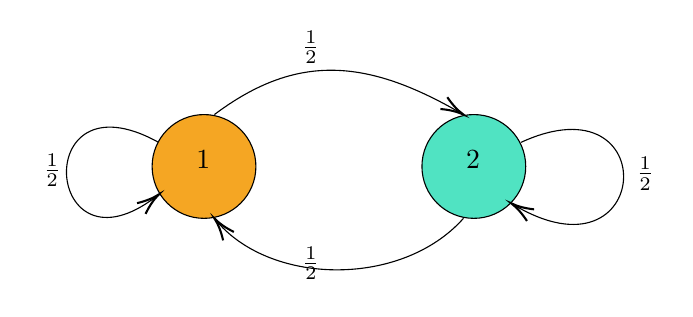
\begin{tikzpicture}[x=0.75pt,y=0.75pt,yscale=-1,xscale=1]
	%uncomment if require: \path (0,300); %set diagram left start at 0, and has height of 300
	
	%Shape: Circle [id:dp10052394937221254] 
	\draw  [fill={rgb, 255:red, 245; green, 166; blue, 35 }  ,fill opacity=1 ] (110,105) .. controls (110,91.19) and (121.19,80) .. (135,80) .. controls (148.81,80) and (160,91.19) .. (160,105) .. controls (160,118.81) and (148.81,130) .. (135,130) .. controls (121.19,130) and (110,118.81) .. (110,105) -- cycle ;
	%Shape: Circle [id:dp9437193586251307] 
	\draw  [fill={rgb, 255:red, 80; green, 227; blue, 194 }  ,fill opacity=1 ] (240,105) .. controls (240,91.19) and (251.19,80) .. (265,80) .. controls (278.81,80) and (290,91.19) .. (290,105) .. controls (290,118.81) and (278.81,130) .. (265,130) .. controls (251.19,130) and (240,118.81) .. (240,105) -- cycle ;
	%Curve Lines [id:da17352138739767575] 
	\draw    (140,80) .. controls (179.6,50.3) and (213.32,53.02) .. (258.62,79.2) ;
	\draw [shift={(260,80)}, rotate = 210.34] [color={rgb, 255:red, 0; green, 0; blue, 0 }  ][line width=0.75]    (10.93,-3.29) .. controls (6.95,-1.4) and (3.31,-0.3) .. (0,0) .. controls (3.31,0.3) and (6.95,1.4) .. (10.93,3.29)   ;
	%Curve Lines [id:da2659131152083798] 
	\draw    (141.59,131.91) .. controls (168.23,162.45) and (230.6,163.07) .. (260,130) ;
	\draw [shift={(140,130)}, rotate = 51.62] [color={rgb, 255:red, 0; green, 0; blue, 0 }  ][line width=0.75]    (10.93,-3.29) .. controls (6.95,-1.4) and (3.31,-0.3) .. (0,0) .. controls (3.31,0.3) and (6.95,1.4) .. (10.93,3.29)   ;
	%Curve Lines [id:da5459168562000609] 
	\draw    (113,93.33) .. controls (50.31,58.59) and (57.92,161.7) .. (112.51,119.07) ;
	\draw [shift={(113.33,118.41)}, rotate = 141.3] [color={rgb, 255:red, 0; green, 0; blue, 0 }  ][line width=0.75]    (10.93,-3.29) .. controls (6.95,-1.4) and (3.31,-0.3) .. (0,0) .. controls (3.31,0.3) and (6.95,1.4) .. (10.93,3.29)   ;
	%Curve Lines [id:da26931738393220694] 
	\draw    (287.67,93.41) .. controls (356.99,61.57) and (351.39,163.71) .. (284.02,123.36) ;
	\draw [shift={(283,122.74)}, rotate = 31.58] [color={rgb, 255:red, 0; green, 0; blue, 0 }  ][line width=0.75]    (10.93,-3.29) .. controls (6.95,-1.4) and (3.31,-0.3) .. (0,0) .. controls (3.31,0.3) and (6.95,1.4) .. (10.93,3.29)   ;
	
	% Text Node
	\draw (130,96) node [anchor=north west][inner sep=0.75pt]   [align=left] {1};
	% Text Node
	\draw (260,96) node [anchor=north west][inner sep=0.75pt]   [align=left] {2};
	% Text Node
	\draw (56.33,97.73) node [anchor=north west][inner sep=0.75pt]   {$\frac{1}{2}$};
	% Text Node
	\draw (342,99.4) node [anchor=north west][inner sep=0.75pt]  {$\frac{1}{2}$};
	% Text Node
	\draw (181,38.4) node [anchor=north west][inner sep=0.75pt]  {$\frac{1}{2}$};
	% Text Node
	\draw (181,142.4) node [anchor=north west][inner sep=0.75pt]   {$\frac{1}{2}$};
	
	
\end{tikzpicture}
\end{figure}\\
	In this example, the state space is $S = \{0,1\}$, and the sample space is
	\[ \Omega = \{ (x_1,x_2,\cdots): x_i \in S \} \]
	which is basically the set of all sequences of one's and zero's. Given this, the random variables $(X_n)_n$ defined t be
	\[  X_n (\omega) = x_n, \]  
	where $\omega \in \Omega$ and $x_n$ is the $n$-th letter in $\omega$. Intuitively speaking, we know that 
	\[  P(1,0) = \prob(X_{n+1} = 1 | X_n = 0) = \frac{1}{2}. \]
	However, here we want to derive that number more explicitly by working directly with the elements of the probability space. First, we need to determine the event associated with $X_{n+1} = 1$. This is the event that has elements where the $n+1$-th position is 1. I.e.
	\[  E = \{  (x_1,x_2, \cdots, x_n, 1, x_{n+2}, \cdots) : x_i \in S\}.  \]
	Similarly, we have
	\[ F = \{ (x_1,x_2, \cdots, x_{n-1},0,x_{n+1},\cdots): x_i \in S \}. \]
	So we have
	\[ \prob(X_{n+1} = 1 | X_n = 0)  = \prob(E|F) = \frac{\prob(E\cap F)}{\prob(F)} =\frac{\prob(E\cap F)}{\prob(F\cap E) + \prob(F\cap E^c)} = \frac{\frac{1}{\abs{\Omega}}}{\frac{1}{\abs{\Omega}} + \frac{1}{\abs{\Omega}}} = \frac{1}{2}. \]
	Note that $\prob(E\cap F) = \frac{1}{\abs{\Omega}}$, since out of many combinations of the sequence of zeros and ones, there is one one sequence whose $n$-th place is 0 and $n+1$-th place is 1. Furthermore, $\prob(F\cap E^c) = \frac{1}{\abs{\Omega}}$ as there is only one string where its $n$-th and $(n+1)$-th string are both zero. 
\end{example}

\begin{example}[Gambler's Ruin]
	Suppose Alice and Bob have in total of $N$ coins. Alice and Bob play a game with a fair coin. When Alice wins, gets a coin from Bop, and vise versa. What is the probability that Alice wins if she starts with $0\leq a \leq N$ coins.
	
	\begin{solution}
		There are many ways to tackle a probability problem like this and the solution presented here is not the only way to find the solution to this problem. We want to model this with Markov chain whose state space is $\{0,1,2,\cdots,N\}$. Thus $X_n$ represents the fortune of Alice after playing the games for $n$ times. 
		\begin{figure}[h!]
	\centering
	
	
	
	\tikzset{every picture/.style={line width=0.75pt}} %set default line width to 0.75pt        
	
	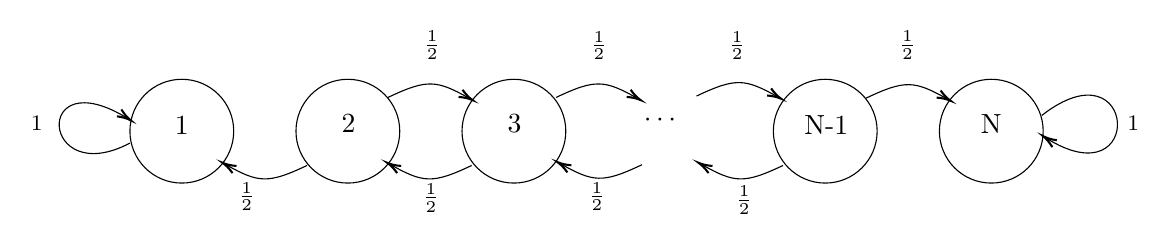
\begin{tikzpicture}[x=0.75pt,y=0.75pt,yscale=-1,xscale=1]
		%uncomment if require: \path (0,300); %set diagram left start at 0, and has height of 300
		
		%Shape: Circle [id:dp09774088338298847] 
		\draw   (100,125) .. controls (100,111.19) and (111.19,100) .. (125,100) .. controls (138.81,100) and (150,111.19) .. (150,125) .. controls (150,138.81) and (138.81,150) .. (125,150) .. controls (111.19,150) and (100,138.81) .. (100,125) -- cycle ;
		%Shape: Circle [id:dp43482816564378113] 
		\draw   (180,125) .. controls (180,111.19) and (191.19,100) .. (205,100) .. controls (218.81,100) and (230,111.19) .. (230,125) .. controls (230,138.81) and (218.81,150) .. (205,150) .. controls (191.19,150) and (180,138.81) .. (180,125) -- cycle ;
		%Shape: Circle [id:dp7628960050576648] 
		\draw   (260,125) .. controls (260,111.19) and (271.19,100) .. (285,100) .. controls (298.81,100) and (310,111.19) .. (310,125) .. controls (310,138.81) and (298.81,150) .. (285,150) .. controls (271.19,150) and (260,138.81) .. (260,125) -- cycle ;
		%Shape: Circle [id:dp3849023603262607] 
		\draw   (410,125) .. controls (410,111.19) and (421.19,100) .. (435,100) .. controls (448.81,100) and (460,111.19) .. (460,125) .. controls (460,138.81) and (448.81,150) .. (435,150) .. controls (421.19,150) and (410,138.81) .. (410,125) -- cycle ;
		%Shape: Circle [id:dp902561209940324] 
		\draw   (490,125) .. controls (490,111.19) and (501.19,100) .. (515,100) .. controls (528.81,100) and (540,111.19) .. (540,125) .. controls (540,138.81) and (528.81,150) .. (515,150) .. controls (501.19,150) and (490,138.81) .. (490,125) -- cycle ;
		%Curve Lines [id:da2277389625716164] 
		\draw    (224.33,108.74) .. controls (243.31,99.74) and (247.7,100.35) .. (263.26,109.02) ;
		\draw [shift={(265,110)}, rotate = 209.42] [color={rgb, 255:red, 0; green, 0; blue, 0 }  ][line width=0.75]    (6.56,-1.97) .. controls (4.17,-0.84) and (1.99,-0.18) .. (0,0) .. controls (1.99,0.18) and (4.17,0.84) .. (6.56,1.97)   ;
		%Curve Lines [id:da8597065575180056] 
		\draw    (305.33,108.74) .. controls (324.31,99.74) and (328.7,100.35) .. (344.26,109.02) ;
		\draw [shift={(346,110)}, rotate = 209.42] [color={rgb, 255:red, 0; green, 0; blue, 0 }  ][line width=0.75]    (6.56,-1.97) .. controls (4.17,-0.84) and (1.99,-0.18) .. (0,0) .. controls (1.99,0.18) and (4.17,0.84) .. (6.56,1.97)   ;
		%Curve Lines [id:da07306821532750352] 
		\draw    (454.67,109.08) .. controls (473.65,100.07) and (478.03,100.69) .. (493.59,109.36) ;
		\draw [shift={(495.33,110.33)}, rotate = 209.42] [color={rgb, 255:red, 0; green, 0; blue, 0 }  ][line width=0.75]    (6.56,-1.97) .. controls (4.17,-0.84) and (1.99,-0.18) .. (0,0) .. controls (1.99,0.18) and (4.17,0.84) .. (6.56,1.97)   ;
		%Shape: Boxed Bezier Curve [id:dp2584084656510479] 
		\draw    (185.33,141.51) .. controls (166.35,150.51) and (161.97,149.9) .. (146.41,141.23) ;
		\draw [shift={(144.67,140.25)}, rotate = 29.42] [color={rgb, 255:red, 0; green, 0; blue, 0 }  ][line width=0.75]    (6.56,-1.97) .. controls (4.17,-0.84) and (1.99,-0.18) .. (0,0) .. controls (1.99,0.18) and (4.17,0.84) .. (6.56,1.97)   ;
		%Shape: Boxed Bezier Curve [id:dp08231579755337615] 
		\draw    (264.67,141.51) .. controls (245.69,150.51) and (241.3,149.9) .. (225.74,141.23) ;
		\draw [shift={(224,140.25)}, rotate = 29.42] [color={rgb, 255:red, 0; green, 0; blue, 0 }  ][line width=0.75]    (6.56,-1.97) .. controls (4.17,-0.84) and (1.99,-0.18) .. (0,0) .. controls (1.99,0.18) and (4.17,0.84) .. (6.56,1.97)   ;
		%Shape: Boxed Bezier Curve [id:dp9912054198682547] 
		\draw    (346.67,141.17) .. controls (327.69,150.18) and (323.3,149.56) .. (307.74,140.89) ;
		\draw [shift={(306,139.92)}, rotate = 29.42] [color={rgb, 255:red, 0; green, 0; blue, 0 }  ][line width=0.75]    (6.56,-1.97) .. controls (4.17,-0.84) and (1.99,-0.18) .. (0,0) .. controls (1.99,0.18) and (4.17,0.84) .. (6.56,1.97)   ;
		%Shape: Boxed Bezier Curve [id:dp49752798194307046] 
		\draw    (414.67,141.51) .. controls (395.69,150.51) and (391.3,149.9) .. (375.74,141.23) ;
		\draw [shift={(374,140.25)}, rotate = 29.42] [color={rgb, 255:red, 0; green, 0; blue, 0 }  ][line width=0.75]    (6.56,-1.97) .. controls (4.17,-0.84) and (1.99,-0.18) .. (0,0) .. controls (1.99,0.18) and (4.17,0.84) .. (6.56,1.97)   ;
		%Curve Lines [id:da6769266285825299] 
		\draw    (373,108.08) .. controls (391.98,99.07) and (396.37,99.69) .. (411.93,108.36) ;
		\draw [shift={(413.67,109.33)}, rotate = 209.42] [color={rgb, 255:red, 0; green, 0; blue, 0 }  ][line width=0.75]    (6.56,-1.97) .. controls (4.17,-0.84) and (1.99,-0.18) .. (0,0) .. controls (1.99,0.18) and (4.17,0.84) .. (6.56,1.97)   ;
		%Curve Lines [id:da5266663507857827] 
		\draw    (539.33,117.41) .. controls (585.53,81.44) and (589.59,158.51) .. (541.47,128.36) ;
		\draw [shift={(540,127.41)}, rotate = 33.33] [color={rgb, 255:red, 0; green, 0; blue, 0 }  ][line width=0.75]    (6.56,-1.97) .. controls (4.17,-0.84) and (1.99,-0.18) .. (0,0) .. controls (1.99,0.18) and (4.17,0.84) .. (6.56,1.97)   ;
		%Curve Lines [id:da13630212552736864] 
		\draw    (100,130.74) .. controls (56.77,153.51) and (52.74,90.36) .. (98.92,118.85) ;
		\draw [shift={(100.33,119.74)}, rotate = 212.76] [color={rgb, 255:red, 0; green, 0; blue, 0 }  ][line width=0.75]    (6.56,-1.97) .. controls (4.17,-0.84) and (1.99,-0.18) .. (0,0) .. controls (1.99,0.18) and (4.17,0.84) .. (6.56,1.97)   ;
		
		% Text Node
		\draw (120.33,116.67) node [anchor=north west][inner sep=0.75pt]   [align=left] {1};
		% Text Node
		\draw (200.67,115.67) node [anchor=north west][inner sep=0.75pt]   [align=left] {2};
		% Text Node
		\draw (280.67,116) node [anchor=north west][inner sep=0.75pt]   [align=left] {3};
		% Text Node
		\draw (423.67,116.33) node [anchor=north west][inner sep=0.75pt]   [align=left] {N-1};
		% Text Node
		\draw (508.67,115.67) node [anchor=north west][inner sep=0.75pt]   [align=left] {N};
		% Text Node
		\draw (151,148.4) node [anchor=north west][inner sep=0.75pt]  [font=\footnotesize]  {$\frac{1}{2}$};
		% Text Node
		\draw (239.67,149.07) node [anchor=north west][inner sep=0.75pt]  [font=\footnotesize]  {$\frac{1}{2}$};
		% Text Node
		\draw (319.67,148.4) node [anchor=north west][inner sep=0.75pt]  [font=\footnotesize]  {$\frac{1}{2}$};
		% Text Node
		\draw (390.67,150.07) node [anchor=north west][inner sep=0.75pt]  [font=\footnotesize]  {$\frac{1}{2}$};
		% Text Node
		\draw (469.33,75.4) node [anchor=north west][inner sep=0.75pt]  [font=\footnotesize]  {$\frac{1}{2}$};
		% Text Node
		\draw (387.33,75.73) node [anchor=north west][inner sep=0.75pt]  [font=\footnotesize]  {$\frac{1}{2}$};
		% Text Node
		\draw (320.67,75.73) node [anchor=north west][inner sep=0.75pt]  [font=\footnotesize]  {$\frac{1}{2}$};
		% Text Node
		\draw (240.33,75.4) node [anchor=north west][inner sep=0.75pt]  [font=\footnotesize]  {$\frac{1}{2}$};
		% Text Node
		\draw (579.33,116.73) node [anchor=north west][inner sep=0.75pt]  [font=\footnotesize]  {$1$};
		% Text Node
		\draw (51,116.4) node [anchor=north west][inner sep=0.75pt]  [font=\footnotesize]  {$1$};
		% Text Node
		\draw (346.33,115.73) node [anchor=north west][inner sep=0.75pt]    {$\cdots $};
		
		
	\end{tikzpicture}
\end{figure} \\
		Let $p_a$ be the probability of Alice wining if she starts with $a$ coins. First, observe that $p_0 = 0$ and $p_N= 1$. Let $E$ denote that event of Alice wining the whole game. Also, let $F_1$ be the event in which she looses the first game and $F_2$ the event in which she wins the first game. Then
		\[ p_a = \prob_a(E) =  \underbrace{\prob_a(E | F_1)}_{\prob(E|F_1,X_0=a)} \prob(F_1) + \underbrace{\prob_a(E|F_1^c)}_{\prob(E|F_1^c,X_0=a)}\prob(F_1^c) \]
		(note that this identity is actually true for any set $F_1$, but here $F_1$ is the specific event explained above). The probability that she looses or wins the first game is $\frac{1}{2}$. Also, observe that $\prob_a(E|F_1) = p_{a+1}$ (since if she wins the first game she will have one more coin) and $\prob_a(E|F_1^c) = p_{a-1}$. Thus 
		\[ p_a = \frac{1}{2}p_{a+1} + \frac{1}{2}p_{a-1}. \]
		Now we can solve this recurrent equation with the characterization polynomial which is $2 = X + 1/X$ or $X^2 - 2X + 1 = (X-1)^2 = 0$. Thus the characteristic polynomial has a double root. Thus 
		\[ p_a = (Aa + B)(1)^a = Aa + B. \]
		Since $p_0 = 0,\ p_N =1$, then it turns out that
		\[ p_a = \frac{a}{N}. \]
	\end{solution}
\end{example}

\begin{example}[Gambler's Ruin with Draw]
	Let Alice and Bob play Rock-Paper-Scissors. If Alice and Bob has a total of $N$ coins, and at each play, the winner gets one coin from the loser, what is the probability that Alice will win the game if he starts with $a$ coins. When they draw, then they repeat the game (or equivalently, they play another game without any coins exchange).
	
	\begin{solution}
		We need to do a first step analysis similar to what we did before. Let $E$ be the event that Alice wins the whole game, and the event $F=F_{-1}\cup F_0 \cup F_1$ where
		\begin{quote}
			$F_{-1}$: Alice loses the first game,\\
			$F_0$: Alice draws the first game,\\
			$F_1$: Alice wins the first game.
		\end{quote}
		It is clear that $\prob(F) = 1$, since the components are mutually disjoint. Thus $E\cap F_{-1},\ E\cap F_0,\ E\cap F_1$ are also mutually disjoints where. Thus we can write
		\[\prob_a(E) = \prob_a(E\cap F_{-1}) + \prob_a(E\cap F_0) + \prob_a(E\cap F_1)
				= \prob_a(E|F_{-1})\prob_a(F_{-1}) + \prob_a(E|F_0)\prob_a(F_0) + \prob_a(E|F_1)\prob_a(F_1).
		\]
		Since the game is fair we know
		\[ \prob_a(F_{-1}) = \prob_a(F_0) = \prob_a(F_1) = \frac{1}{3}.  \]
		Furthermore, we know
		\[ \prob_a(E|F_{-1}) = p_{a-1}, \qquad \prob_a(E|F_0) = p_a, \qquad \prob_a(E|F_1) = p_{a+1}. \]
		Thus the first step analysis will lead to the following identity.
		\[  \prob_a(E) = p_a = \frac{1}{3} ( p_{a-1} + p_{a} + p_{a+1}),\]
		which after simplification becomes
		\[ 2p_a = p_{a-1} + p_{a+1}, \]
		which is the same recursive formula we got in the previous example. So the possibility of the draw, will not change the behaviour of the system.
	\end{solution}
\end{example}


\begin{proposition}[First step argument]
	Let $(X_n)_{n\geq 0}$ be a Markov chain on the state space $S$. Let $x\in S$, and $W,Z \subset S$. Let $B$ be any event. Then
	\[ \prob_x(B) = \sum_{y:x\sim y} \prob_y(B)P(x,y). \]
	\label{prop:FirstTimeStepArgument}
\end{proposition}
\begin{proof}
	To prove the proposition above, we Let $E_i = \{ X_0=x, X_1=y_i \}$ where $y_i \sim x$. So, in words, we say that the event $E_i$ has occurred if $X_1 = y_i$. It is clear that $E_i \cap E_j = \emptyset$ where $i\neq j$. Thus $\bigcup_{i}(B\cap E_i) = B$. Thus 
	\[ \prob_x(B) = \sum_{i} \prob_x(B \cap E_i) = \sum_{i}\prob_x(B|E_i)\prob_x(E_i). \]
	In which $\prob_x(E_i) = \prob(E_i|X_0=x) = \prob(X_1=y_i|X_0=x) = P(x,y_i)  $. Also \[\prob_x(B|E_i) = \prob(B|X_1=y_i, X_0=x) = \prob(B|X_1=y_i) = \prob_{y_i}(B),\].
	in which we have used the Markov property. Thus we can write
	\[ P_x(B) = \sum_i \prob_{y_i}(B)P(x,y_i). \]
\end{proof}


\begin{example}
	Consider the a simple random walker on the following graph. Let $B = \{ T_{\tilde{x}} < T_{\set{\tilde{z},\tilde{y}}} \}$. Compute the probability $\prob_0(B)$.
	
	\begin{center}
		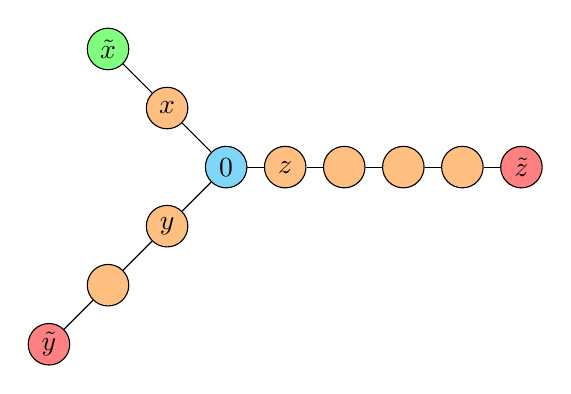
\begin{tikzpicture}[scale=1.5, every node/.style={circle, draw}]
			\tikzstyle{every node}=[circle, draw, fill=white,
			inner sep=0pt, minimum width=15pt]
			
			\node[fill=cyan!50] (a) at (0,0) {0};
			\node[fill=orange!50] (z1) at (1/2,0) {$z$};
			\node[fill=orange!50] (z2) at (2/2,0) {};
			\node[fill=orange!50] (z3) at (3/2,0) {\ };
			\node[fill=orange!50] (z4) at (4/2,0) {\ };
			\node[fill=red!50] (ze) at (5/2,0) {$\tilde{z}$};
			
			\node[fill=orange!50] (x1) at (-1/2,1/2) {$x$};
			\node[fill=green!50] (xe) at (-1,1) {$\tilde{x}$};
			
			\node[fill=orange!50] (y1) at (-1/2,-1/2) {$y$};
			\node[fill=orange!50] (y2) at (-2/2,-2/2) {};
			\node[fill=red!50] (ye) at (-3/2,-3/2) {$\tilde{y}$};
			
			
			\draw (a) -- (z1);
			\draw (z1) -- (z2);
			\draw (z2) -- (z3);
			\draw (z3) -- (z4);
			\draw (z4) -- (ze);
			
			\draw (a) -- (y1);
			\draw (y1) -- (y2);
			\draw (y2) -- (ye);
			
			\draw (a) -- (x1);
			\draw (x1) -- (xe);
			
		\end{tikzpicture}
	\end{center}
	
	\begin{solution}
		This problem is simply asking what is the probability that we hit $\tilde{x}$ state before hitting any of $\tilde{y}$ or $\tilde{z}$ states, given the fact that the random walker starts from the state $0$. To keep unnecessary details out of the way, we have only labeled the vertices that we will use in our analysis. We will have the following notation to simplify the solution
		\[ p_v = \prob_v(B), \]
		where $v$ is any vertex in the graph. Note that starting at 0, i.e. $X_0=0$, then going to any of the states $x,y$, or $z$, are mutually disjoint events, and the probability of the union of these events is one. With our first time step analysis (see \autoref{prop:FirstTimeStepArgument}) we can write
		\[ \prob_0(B) = \frac{1}{3} ( p_x + p_y + p_z). \]
		Now we need to analyze each of terms in the RHS. Let's start with $p_z$. Consider two events $\{ T_0 < T_{\tilde{z}}  \}$ and $\{ T_0 > T_{\tilde{z}}  \}$, where the first time is the event where the random walker hits the $0$ state before hitting the $\tilde{z}$ step first, and the second one is the vice versa. These two events are disjoint and the probability of the union is 1. Thus we write the conditional expansion of $p_z$ based on these events
		\[ p_z = \prob_z(B) = \prob_z(B|T_0 < T_{\tilde{z}})\prob_z(T_0 < T_{\tilde{z}}) + \prob_z(B|T_0 > T_{\tilde{z}})\prob_z(T_0 > T_{\tilde{z}}). \]
		We know that $\prob_z(B|T_0 > T_{\tilde{z}}) = \prob(B|X_0=z,X_i=\tilde{z})$ for some $i > 0$. From Markov property it follows that 
		\[ \prob(B|X_0=z,X_i=\tilde{z}) = \prob(B|X_i=\tilde{z}) = \prob(B|X_0 = \tilde{z})  = p_{\tilde{z}}.\]
		Also $\prob_z(B|T_0<T_{\tilde{z}}) = \prob_0(B) = p_0$ by the Markov property. Lastly, $\prob_z(T_0<T_{\tilde{z}})$ is determined by the Gambler's ruin method we say before, which is basically
		\[ \prob_z(T_0 < T_{\tilde{z}}) = \frac{5}{4}, \qquad \prob_z(T_0>T_{\tilde{z}}) = \frac{1}{5}. \]
		By doing the same kind of analysis for $p_x$ as well as $p_y$ we will get
		\[ p_z = \frac{4}{5}p_0 , \qquad p_y = \frac{2}{3}p_0, \qquad p_x =\frac{1}{2}p_0 + \frac{1}{2}. \]
		Now by substituting in the identity we got from the first time step argument, we can fine that 
		\[ p_0 = \frac{15}{31}, \]
		And this completes our solution for the problem.
	\end{solution}
	
\end{example}

\begin{example}
	Consider the graph $\gamma=  (V,E)$ drawn below. Set $Z = \{2,3\}$, and $W = \set{6,9}$. Compute $\prob_0(T_Z<T_W)$. In colors: we start at blue, win if we reach green, and lose of we reach red.
	
	\begin{center}
		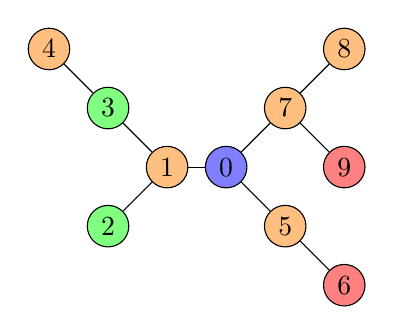
\begin{tikzpicture}[scale=1.5, every node/.style={circle, draw}]
			\tikzstyle{every node}=[circle, draw, fill=orange!50,
			inner sep=0pt, minimum width=15pt]
			
			\node[fill=blue!50] (n0) at (1/2,0) {0};
			\node (n1) at (0/2,0) {1};
			\node[fill=green!50] (n2) at (-1/2,-1/2) {2};
			\node[fill=green!50] (n3) at (-1/2,1/2) {3};
			\node (n4) at (-2/2,2/2) {4};
			\node (n5) at (2/2,-1/2) {5};
			\node[fill=red!50] (n6) at (3/2,-2/2) {6};
			\node (n7) at (2/2,1/2) {7};
			\node (n8) at (3/2,2/2) {8};
			\node[fill=red!50] (n9) at (3/2,0/2) {9};

			
			\draw (n0) -- (n1);
			\draw (n1) -- (n2);
			\draw (n1) -- (n3);
			\draw (n3) -- (n4);
			\draw (n0) -- (n7);
			\draw (n0) -- (n5);
			\draw (n5) -- (n6);
			\draw (n7) -- (n9);
			\draw (n7) -- (n8);
			
		\end{tikzpicture}
	\end{center}
\end{example}

\begin{solution}
	As always, we start with our powerful tool in hand, which is the first step argument (which is basically a special form of the more general conditional expansion). We start with first step argument at state $0$. We will get
	\[ \prob_0(B) = \frac{1}{3} (\prob_1(B) + \prob_7(B) + \prob_5(B) ), \]
	and now we need to analyze each of the terms in the right hand side. We start with $\prob_5(B)$ which is the most straight forward one. As we saw in the last example, we can analyze this state with a conditional expansion on the two disjoint events, whose union probability is 1. Let those two events be $\set{T_6 < T_0}$ (where the random walker hits the state $6$ before hitting the state $0$), and $\set{T_6 > T_0}$, where the random walker hits the state $0$ before hitting the state $6$. Thus the expansion will be
	\[ \prob_5(B) = \prob_5(B|T_6 < T_0) \prob_5(T_6 < T_0) + \prob_5(B|T_6 > T_0)\prob_5(T_6 > T_0). \]
	We know that if we hit the state $6$ before $0$, we have no chance to hit any of the green states (we will lose). Thus
	\[ \prob_5(B|T_6<T_0) = 0. \]
	And from the Gambler's ruin we know that $\prob_5(T_6>T_0) = 1/2$, and from the Markov property we know that $\prob_5(B|T_6>T_0) = \prob_0(B)$, because the conditional probability $\prob_5(B|T_6>T_0)$ is basically stating what is the probability of $B$ happening, if we start from $5$ and $X_i = 0$ for some $i$ in the future. Thus 
	\[ \prob_5(B) = \frac{\prob_0(B)}{2}. \]
	Now, we need to analyze the term $\prob_1(B)$. Again, at this step, we do another first step analysis.
	\[  \prob_1(B) = \frac{1}{3} (\underbrace{\prob_3(B)}_{=1} + \underbrace{\prob_2(B)}_{=1} +\prob_0(B)) = \frac{2+\prob_0(B)}{3}. \]
	Note that from the assumption, we know that if we reach any of green states, then we are declared winner, that is why we have $\prob_3(B) = \prob_2(B) = 1$. Now it only remains to analyze the term $\prob_7(B)$. Again, similar to the case above, we do a first time step argument
	\[ \prob_7(B) = \frac{1}{3} ( \prob_0(B) + \underbrace{\prob_8(B)}_{=\prob_7(B)} + \underbrace{\prob_9(B)}_{=0} ) \implies \prob_7(B) = \frac{\prob_0(B)}{2}.\]
	Note that $\prob_8(B) = \prob_7(B)$ by a first stem analysis when starting at the state $8$. Putting all of these terms back to the original identity we derived the first, we can conclude that 
	\[ p_0 = \prob_0(B) = \frac{2}{5}. \]
\end{solution}




\section{Solved Problems}
\begin{question} 
	If $A, B$ and $C$ are sets. prove the followings:
	\begin{enumerate}[(a)]
		\item $A \cap (B \cup C) = (A \cap B) \cup (A \cap C)$. \label{section-a}
		\item $C \textbackslash (A \cup B) = (C \textbackslash A) \cap (C \backslash B)$.
		
		\item $C \backslash (A \cap B) = (C \backslash A) \cup (C \backslash B) $.
		
	\end{enumerate}
	
	\begin{ans}
		\begin{enumerate}[(a)]
			\item 
			\begin{proof}
			Let $P, Q$, and $R$ be logical statements. We can show (using the truth table) that the following biconditional implication is a tautology. \[ P \wedge (Q \vee R) \Leftrightarrow (P \wedge Q) \vee (P \wedge R). \]
			Now let $x \in A \cap (B \cup C)$. Then $x \in A \wedge (x \in B \vee x \in C)$. Using the tautology above we can write $(x \in A \wedge x \in B) \vee (x \in A \wedge x \in C)$, thus $x \in (A \cap B) \cup (A \cap C) $, which means $A \cap (B \cap C) \subset (A \cap B) \cup (A \cap C)$. Conversely, let $x \in (A \cap B) \cup (A \cap C)$. By definition $(x \in A \wedge x \in B) \vee (x \in A \wedge x \in C)$. With the similar logic as above we can infer $(A \cap B) \cup (A \cap C) \subset A \cap (B \cup C)$. Thus $A \cap (B \cup C) = (A \cap B) \cup (A \cap C)$.
			\end{proof}
			
			\item 
			\begin{proof}
			Let $x \in C \backslash (A \cup B)$. By definition $x \in C \wedge x \notin (A \cup B) \biImp x \in C \wedge x \in \overline{A \cup B} \biImp x \in C \wedge x \in \bar{A} \cap \bar{B} \biImp x \in C \wedge (x \notin A \wedge x \notin B)$. Finally, using the following tautology 
			\[ P \wedge (Q \wedge R) \Leftrightarrow (P \wedge Q) \wedge (P \wedge R), \]
			we can write $(x \in C \wedge x \notin A) \wedge (x \in C \wedge x \notin B) \biImp x \in (C \backslash A) \cap (C \backslash B) $, thus $C \textbackslash (A \cup B) subset (C \textbackslash A) \cap (C \backslash B)$. The converse can be shown is true following the similar logic as below, thus inferring $C \textbackslash (A \cup B) = (C \textbackslash A) \cap (C \backslash B)$.
			\end{proof}
			
			\item \begin{proof}
			Let $x \in C \backslash (A \cap B)$. By definition $x \in C \wedge x \notin (A \cap B) \biImp x \in C \wedge x \in \overline{A \cap B} \biImp x \in C \wedge x \in \bar{A} \cup \bar{B} \biImp x \in C \wedge (x \notin A \vee x \notin B)$. Using the tautology in section (a),
			we can write $(x \in C \wedge x \notin A) \vee (x \in C \wedge x \notin B) \biImp x \in (C \backslash A) \cup (C \backslash B) $, thus $C \textbackslash (A \cap B) \subset (C \textbackslash A) \cup (C \backslash B)$. The converse can be shown is true following the similar logic as below, thus inferring $C \textbackslash (A \cap B) = (C \textbackslash A) \cup (C \backslash B)$.
			\end{proof}
			
			
			
			
		\end{enumerate}
	\end{ans}
\end{question}
\begin{problem}
	There are 6 coins on a table, each showing heads (H) or tails (T). In each step we 
	\begin{itemize}
		\item Select uniformly one of the coins. 
		\item If it is heads, toss it and replace on the table (with random side).
		\item If it sis tails, toss it. If it comes up heads, leave it at that. If it comes up tails, toss it a second time, and leave the result as it is.
		Let $X_n$ be the number of heads showing after $n$ such steps. Answer the following questions
		\begin{enumerate}[(a)]
			\item Determine the transition probabilities for this Markov chain.
			\item Draw the transition diagram and write the transition matrix.
			\item What is $\prob(X_2 = 4| X_0=5)$?
		\end{enumerate}
	\end{itemize}
\end{problem}
\begin{solution}
	\begin{enumerate}[(a)]
		\item To compute the transition probabilities, we need to perform the first step analysis. Let the events \[I = \set{X_1 = a+1},\qquad S = \set{X_1 = a},\qquad D = \set{X_1 = a-1},\]
		where $0 \leq a \leq 6$ is the number of heads. So to compute the transition probabilities, we need to compute
		\[ P(a,a+1) = \prob_a(I), \qquad P(a,a) = \prob_a(S), \qquad P(a,a-1) = \prob_a(D). \]
		We start with $\prob_a(I)$. Let $ST$ be the event where the selected coin is tails, and $SH$ be the event where the selected coin is heads. These two events are disjoint and the probability of their union is 1, thus
		\[ \prob_a(I) = \underbrace{\prob_a(I|SH)}_{\text{see Eq (2.I.1)}}\underbrace{\prob_a(SH)}_{\frac{a}{6}} + \underbrace{\prob_a(I|ST)}_{\text{see Eq (2.I.2)}}\underbrace{\prob_a(ST)}_{\frac{6-a}{6}}. \tag{2.I}\]
		Note that if we start with $a$ coins heads, then the chance we choose a random coin from the table and find it heads is $\frac{a}{6}$, hence $\prob_a(SH) = \frac{a}{6}$, and $\prob_a(ST) = \frac{6-a}{6}$. Now we need to expand the remaining terms with appropriate conditioning. Let $TT$ be the event where we toss a coin and find it tails and $TH$ be the event where we toss a coin and find it heads. Thus we can write
		\[ \prob_a(I|SH) = \underbrace{\prob_a(I|SH,TH)}_{0}\underbrace{\prob_a(TS)}_\frac{1}{2} + \underbrace{\prob_a(I|SH,TT)}_{0}\underbrace{\prob_a(TT)}_\frac{1}{2}. \tag{2.I.1}  \]
		Note that $\prob_a(TT) = \prob_a(TH) = \frac{1}{2}$, since the coin tossing is fair. Also, note that $\prob_a(I|SH,TH)=\prob_a(I|SH,TT)=0$ since if we select a heads, and then toss it, finding it either heads or tails will not increase the total number of heads on the table. Similarly, for the other term in $(2.1)$ we have
		\[ \prob_a(I|ST) = \underbrace{\prob_a(I|ST,TH)}_{1}\underbrace{\prob_a(TH)}_{\frac{1}{2}} + \underbrace{\prob_a(I|ST,TT)}_\text{see Eq (2.I.3)}\underbrace{\prob_a(TT)}_{\frac{1}{2}}. \tag{2.I.2} \]
		Now we need to expand the remaining terms in the equation above.
		\[ \prob_a(I|ST,TT) = \underbrace{\prob_a(I|ST,TT,TH)}_{1}\prob_a(TH) + \underbrace{\prob_a(I|ST,TT,TT)}_{0}\prob_a(TT) = \frac{1}{2}. \tag{2.I.3}  \]
		Putting all together we can write
		\[ \boxed{P(a,a+1) = \prob_a(I) = \frac{6-a}{8}}. \]
		Similarly, we can compute other transition probabilities. For instance for $\prob_a(S)$ we can write
		\[ \prob_a(S) = \underbrace{\prob_a(S|SH)}_{\text{see Eq (2.S.1)}}\underbrace{\prob_a(SH)}_{\frac{a}{6}} + \underbrace{\prob_a(S|ST)}_{\text{see Eq (2.S.2)}}\underbrace{\prob_a(ST)}_{\frac{6-a}{6}}. \tag{2.S}\]
		and for the remaining terms we can write
		\[ \prob_a(S|SH) = \underbrace{\prob_a(S|SH,TH)}_{1}\underbrace{\prob_a(TS)}_\frac{1}{2} + \underbrace{\prob_a(S|SH,TT)}_{0}\underbrace{\prob_a(TT)}_\frac{1}{2}, \tag{2.S.1}  \]
		and
		\[ \prob_a(S|ST) = \underbrace{\prob_a(S|ST,TH)}_{0}\underbrace{\prob_a(TH)}_{\frac{1}{2}} + \underbrace{\prob_a(S|ST,TT)}_\text{see Eq (2.S.3)}\underbrace{\prob_a(TT)}_{\frac{1}{2}}. \tag{2.S.2} \]
		And for the remaining term above
		\[ \prob_a(S|ST,TT) = \underbrace{\prob_a(S|ST,TT,TH)}_{0}\prob_a(TH) + \underbrace{\prob_a(S|ST,TT,TT)}_{1}\prob_a(TT) = \frac{1}{2}. \tag{2.S.3}  \]
		and by putting all together we will get
		\[\boxed{ P(a,a) =  \prob_a(S) = \frac{6+a}{24}}. \]
		Finally, since $\prob_a(I\cup S \cup D) = 1$, and $I,S,D$ are mutually disjoint, we can write 
		\[ \prob_a(D) = 1 - (\prob_a(I) + \prob_a(S)), \] 
		hence
		\[ \boxed{P(a,a-1) = \prob_a(D) = \frac{a}{12}}. \]
		so the transition probabilities are as calculated.
		
		\item The transition diagram is plotted below. 
		
		\begin{center}
			\begin{tikzpicture}[->,>=stealth',shorten >=1pt,auto,node distance=1.9cm,
				semithick,scale=0.4]
				\tikzstyle{every state}=[circle, draw, fill=orange!50,
				inner sep=0pt, minimum width=10pt]
				
				\node[state] (A)              {$0$};
				\node[state]         (B) [right of=A] {$1$};
				\node[state]         (C) [right of=B] {$2$};
				\node[state]         (D) [right of=C] {$3$};
				\node[state]         (E) [right of=D] {$4$};
				\node[state]         (F) [right of=E] {$5$};
				\node[state]         (G) [right of=F] {$6$};
				
				\path (A) edge [bend left] node {$p_{01}$} (B)
				(B) edge [bend left] node {$p_{10}$} (A)
				(A) edge [loop left] node {$p_{00}$} (A)
 				
				(B) edge [bend left] node {$p_{12}$} (C)
				(B) edge [loop above] node {$p_{11}$} (C)
				(C) edge [bend left] node {$p_{21}$} (B)
				
				(C) edge [bend left] node {$p_{23}$} (D)
				(C) edge [loop below] node {$p_{22}$} (D)
				(D) edge [bend left] node {$p_{32}$} (C)
				
				(D) edge [bend left] node {$p_{34}$} (E)
				(D) edge [loop above] node {$p_{33}$} (E)
				(E) edge [bend left] node {$p_{43}$} (D)
				
				(E) edge [bend left] node {$p_{45}$} (F)
				(E) edge [loop below] node {$p_{44}$} (E)
				(F) edge [bend left] node {$p_{54}$} (E)
				
				(F) edge [bend left] node {$p_{56}$} (G)
				(F) edge [loop above] node {$p_{55}$} (E)
				(G) edge [bend left] node {$p_{65}$} (F)
				(G) edge [loop right] node {$p_{66}$} (G);
			\end{tikzpicture}
		\end{center}
		And the transition matrix is
		\[  M =
		\begin{pmatrix}
			1/4 & 3/4 & 0 & 0 & 0 & 0 & 0 \\
			1/12 & 7/24 & 5/8 & 0 & 0 & 0 & 0 \\
			0 & 1/6 & 1/3 & 1/2 & 0 & 0 & 0 \\
			0 & 0 & 1/4 & 3/8 & 3/8 & 0 & 0 \\
			0 & 0 & 0 & 1/3 & 5/12 & 1/4 & 0 \\
			0 & 0 & 0 & 0 & 5/12 & 11/24 & 1/8 \\
			0 & 0 & 0 & 0 & 0 & 1/2 & 1/2
		\end{pmatrix}
		 \]
		 
		 \item $\prob(X_2 = 4|X_0=5)$ is the second transition probability $P_2(5,4)$. To compute this, we need to fine the element in the 6-th row and 5-th column in the $M^2$ matrix, which is basically the inner product between the vectors formed by the 6-th row and the 5-th column.
		 \[ P_2(5,4) = (\frac{5}{12})^2 + \frac{11}{24}\cdot\frac{5}{12} = \frac{35}{96} \]
		 which after simplification becomes
		 \[ \boxed{P_2(5,4) = \frac{35}{96}}. \]
		\qed

		
		
		
	\end{enumerate}
	
\end{solution}
\begin{question}
	A clock is broken. It has only one hand which moves every hour either clockwise with probability 1/2 or counter-clockwise with probability 1/2 (the numbers are from 0 to 11 and the hand moves by one full hour when it moves). Assume it starts at 0. What is the probability that it reaches 7 before coming back to 0 for the first time?
\end{question}
\begin{ans}
	First, let's draw the graph representing the state space of the random variable of interest.
	\begin{center}
		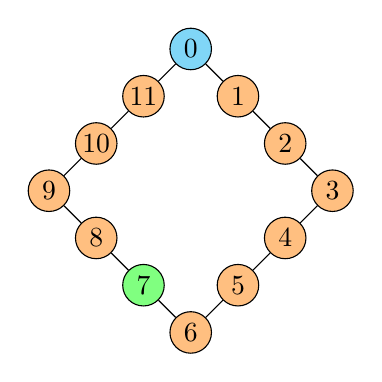
\begin{tikzpicture}[scale=0.6, every node/.style={circle, draw}]
			\tikzstyle{every node}=[circle, draw, fill=orange!50,
			inner sep=0pt, minimum width=15pt]
			
			
			\node[fill=cyan!50] (n0) at (0,3) {0};
			\node (n1) at (1,2) {1};
			\node (n2) at (2,1) {2};
			\node (n3) at (3,0) {3};
			\node (n4) at (2,-1) {4};
			\node (n5) at (1,-2) {5};
			\node (n6) at (0,-3) {6};
			
			\node (n11) at (-1,2) {11};
			\node (n10) at (-2,1) {10};
			\node (n9) at (-3,0) {9};
			\node (n8) at (-2,-1) {8};
			\node[fill=green!50] (n7) at (-1,-2) {7};
			
		
			\draw (n0) -- (n1);
			\draw (n1) -- (n2);
			\draw (n2) -- (n3);
			\draw (n3) -- (n4);
			\draw (n4) -- (n5);
			\draw (n5) -- (n6);
			\draw (n6) -- (n7);
			\draw (n7) -- (n8);
			\draw (n8) -- (n9);
			\draw (n9) -- (n10);
			\draw (n10) -- (n11);
			\draw (n11) -- (n0);
			
		\end{tikzpicture}
	\end{center}
	
	Define the event $B$ be $B = \set{T^+_0 > T_7}$. We are interested in finding $\prob_0(B)$. Now we can perform the first step argument as follows
	\[ p_0 = \frac{1}{2}(p_1 + p_{11}). \tag{3.1} \]
	Then we analyze each term in the right hand side of the equation above. For $p_1$ we have
	\[ \prob_1(B) = \underbrace{\prob_1(B|T_0>T_7)}_{1}\underbrace{\prob_1(T_0>T_7)}_{1/5} + \underbrace{\prob_1(B|T_0<T_7)}_{0}\underbrace{\prob_1(T_0<T_7)}_{6/7} = \frac{1}{5}. \]
	Note that $\prob_1(B|T_0>T_7)=1$ since it literally means the random walker reaches 7 before 0. Also $\prob_1(B|T_0<T_7)=0$ since the event $B$ is conditioned on reaching 0 before 7, which is clearly 0. The term $\prob_1(T_0>T_7)$ is computed using the Gambler's ruin analysis. Similarly, for the $p_{11}$ term we have
	\[ \prob_{11}(B) = \underbrace{\prob_{11}(B|T_0>T_7)}_{1}\underbrace{\prob_{11}(T_0>T_7)}_{1/7} + \underbrace{\prob_{11}(B|T_0<T_7)}_{0}\prob_{11}(T_0<T_7) = \frac{1}{7}. \]
	The rationale behind the values of the terms are the same as the ones discussed above. Now we can substitute everything in $(3.1)$
	\[ \boxed{p_0 = \frac{1}{2} (\frac{12}{35}) = \frac{6}{35}}. \]
	
\end{ans}
\begin{question}
	The Fibonacci sequence is the sequence $(F_n)_{n\geq0}$ defined by $F_0 = 0, F_1=1$ and 
	\[ F_{n+2} = F_{n+1} + F_n \quad \text{for } n\geq 0.  \]
	Find a general formula for $F_n$
\end{question}
\begin{ans}
	First, we construct the characteristic polynomial of the sequence. From the recursive formula we can write
	\[ X^2 = X + 1 \implies \boxed{X^2 - X - 1 = 0}. \]
	The roots of the equation is 
	\[ r_1, r_2 = \frac{1 \pm \sqrt{5}}{2}. \]
	Now the general formula will be
	\[ F_n = Ar_1^n + Br_2^n. \] 
	To find the coefficients, we utilize the first two terms 
	\[ 0 = A + B, \qquad 1 = \frac{1}{2}(A+B) + \frac{\sqrt{5}}{2}(A-B). \]
	This system of equations implies that
	\[ A = \frac{1}{\sqrt{5}}, \qquad B=\frac{-1}{\sqrt{5}}.  \]
	Thus the general formula will be
	\[ \boxed{F_n = \frac{1}{\sqrt{5}}((\frac{1+\sqrt{5}}{2})^n - \frac{1-\sqrt{5}}{2})^n)}. \]
	
	\qed
	
\end{ans}
\begin{question}
	Let $(X_n)$ be the simple random walk on the following graph. Compute $\prob_0(T_3<T_7)$.
	
	\begin{center}
		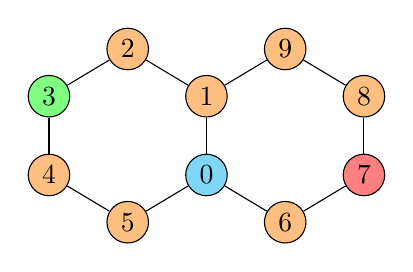
\begin{tikzpicture}[scale=1, every node/.style={circle, draw}]
			\tikzstyle{every node}=[circle, draw, fill=orange!50,
			inner sep=0pt, minimum width=15]
			
			
			\node[fill=cyan!50] (n0) at (0,0) {0};
			\node (n1) at (0,1) {1};
			\node (n2) at (-1,1.6) {2};
			\node[fill=green!50] (n3) at (-2,1) {3};
			\node (n4) at (-2,0) {4};
			\node (n5) at (-1,-0.6) {5};
			\node (n9) at (1,1.6) {9};
			\node (n8) at (2,1) {8};
			\node[fill=red!50] (n7) at (2,0) {7};
			\node (n6) at (1,-0.6) {6};

			\draw (n0) -- (n1);
			\draw (n1) -- (n2);
			\draw (n2) -- (n3);
			\draw (n3) -- (n4);
			\draw (n4) -- (n5);
			\draw (n5) -- (n0);
			\draw (n0) -- (n6);
			\draw (n6) -- (n7);
			\draw (n7) -- (n8);
			\draw (n8) -- (n9);
			\draw (n9) -- (n1);

			
		\end{tikzpicture}
	\end{center}
\end{question}
\begin{ans}
	For a much more simpler solution, let's define the two following notations
	\[ B = \{T_3 < T_7\}, \qquad p_v = \prob_v(B). \]
	Then, by first step argument at state $0$, we can write
	\[ p_0 = \frac{1}{3} (p_5 + p_6 + p_1).  \tag{5.1}\]
	Now we need to evaluate each of the terms in the right hand side. We start with $p_5$.
	\[ p_5 = \prob_5(B) = \underbrace{\prob_5(B|T_3<T_0)}_{1}\underbrace{\prob_5(T_3<T_0)}_{1/3} + \underbrace{\prob_5(B|T_3>T_0)}_{p_0}\underbrace{\prob_5(T_3>T_0)}_{2/3} = \frac{1}{3} + \frac{2}{3}p_0. \]
	note that $\prob_5(B|T_3<T_0) = 1$, since if we get to state 3, before getting to state 0, then it means that we have reached the state 3 before reaching the state 7, thus the event $B$ occurs with probability 1. Also $\prob_5(T_3<T_0) = 1/3$ from the Gambler's ruin. Furthermore $\prob_5(B|T_3>T_0) = p_0$ by using the Markov property, and finally $\prob_5(T_3>T_0) = 2/3$ by the Gambler's ruin. \\
	Now, we need to evaluate the term $p_6$. To analyze this term, we will do a first step argument starting at this point
	\[ p_6 = \prob_6(B) = \frac{1}{2}(\underbrace{p_7}_{0} + p_0) = \frac{p_0}{2}. \]
	Note that $p_7 = 0$, since then the event $B$ has not occurred. \\
	Finally, we need to analyze the term $p_1$. Again, by first step argument on this state we have
	\[ p_1 = \frac{1}{3}(p_0 + p_9 + p_2). \]	
	By doing a analysis on $p_9$ similar to the one we did for 5, we can write
	\[ p_9 = \prob_9(B)= \underbrace{\prob_9(B|T_7<T_1)}_{0}\prob_9(T_7<T_1) + \underbrace{\prob_9(B|T_7>T_1)}_{p_1}\underbrace{\prob_9(T_7>T_1)}_{2/3} = \frac{2}{3}p_1. \]
	The rationale behind the values for each term in the equation above, is exactly the same as in analyzing the terms of $p_5$.\\
	Now, we analyze the term $p_2$ by performing another first step analysis, similar to the one we did for state 6.
	\[ p_2 = \frac{1}{2}(\underbrace{p_3}_1 + p_1) = \frac{1}{2}(1+p_1). \]
	Now we can calculate $p_1$ in terms of $p_0$ which turns out to be
	\[ p_1 = \frac{6}{11}p_0 + \frac{3}{11}.  \]
	Now we insert all of the terms in the equation $(5.1)$ to get
	\begin{align*}
		&3p_0 = \frac{1}{3}+\frac{2}{3}p_0 + \frac{1}{2}p_0 + \frac{6}{11}p_0 + \frac{3}{11} \\ 
		&\implies 3p_0 - \frac{113}{66}p_0 = \frac{40}{33} \\
		&\implies p_0 = \frac{66}{85}\cdot\frac{40}{33} = \frac{16}{17}\\
		&\implies \boxed{p_0 = \frac{16}{17}}.
	\end{align*}


	\qed
	
	

\end{ans}


\chapter{Stationary Distributions of Markov Chains}

\section{Time Evolution of Distributions}

Let $ \set{X_n}_n $ be a discrete Markov with finite state space $ S = \set{1,2,\cdots,N} $. Then, we know that starting at a state $ X_0 = 1 $, then the probability to be at state $ j $ after one step is the $ (1,j) $ element of the transition matrix. To be more concrete, let's assume that the Markov chain is defined on $ \set{1,2,3} $, and assume $ X_0 = 1 $. Then $ P(1,3)=\prob_1(X_1=3) $ is the element $ (1,3) $ of the transition matrix. Don't forget that $ \set{X_n} $ are all random variables. Thus while we can talk about the cases that what will happen if, for example $ X_0 $, be $ X_0=1 $ and etc. We can also talk about the probability that the random variable has specific values, which is the idea of distribution. Let $ \mu_{X_0}(i) $ for $ i \in \set{1,2,3} $ be the distribution of $ X_0 $. In other words, we have
\[   \mu_{X_0}(i) = \prob(X_0 = i) \qquad \text{for $ i \in \set{1,2,3}$}.  \]
We can also introduce the vector notation for the distribution. Note that we can drop the subscript $ X_0 $ as shown in the following notation.
\[  \mu_0=\mu_{X_0} = (\mu_{X_0}(1),\mu_{X_0}(2),\mu_{X_0}(3)). \]
Now, suppose we want to find the distribution of $X_1$ given the distribution of $X_0$, i.e. we want to calculate the time evolution of the distribution after one step. Let's calculate what happens for $  \mu_0 $ after one step:
\[  \mu_1 = \mu_{X_1} = (\mu_1(1),\mu_1(2),\mu_1(3)).  \]
To calculate $ \mu_1(1) $ we can write
\[ \mu_1(1) = \prob(X_1 = 1) = \underbrace{\prob_1(X_1 = 1)}_{P(1,1)}\underbrace{\prob(X_0=1)}_{\mu_0(1)} + \underbrace{\prob_2(X_1 = 1)}_{P(2,1)}\underbrace{\prob(X_0=2)}_{\mu_0(2)} +  \underbrace{\prob_3(X_1 = 1)}_{P(3,1)}\underbrace{\prob(X_0=3)}_{\mu_0(3)}. \]
In summary
\[ \mu_1(1) = P(1,1)\mu_0(1) + P(2,1)\mu_0(2) + P(3,1)\mu_0(3). \]
By a similar argument, we can quickly see that
\[  \mu_1 = \mu_0 M  \]
where $ M $ is the transition matrix.
\begin{proposition}
	Let $ X_0 \sim \mu_0 $. Then $ X_n \sim \mu_n $ where
	\[ \mu_n = \mu_0 M^n \]
	where $ M $ is the transition matrix. 
\end{proposition}

Now we can state the following important observation.
\begin{observation}
	For a given discrete Markov chain $ \set{X_n} $ defined on a \emph{finite} state space $ S = \set{1,2,\cdots, N} $, the sequence of distributions of the random variables at each time step
	\[ \mu_{X_n} = \mu_n = (\mu_n(1),\mu_n(2),\cdots,\mu_n(N)), \]
	defines a discrete time Markov chain with continuous state space $ \R^{N-1} $. The transition matrix for $ \set{\mu_n}_n $ will be the same as the original Markov chain. The state space will in fact be an affine hyperplane at $ \R^N $, that intersects each axis at 1. That is because we require the distributions to sum up to 1. Thus we will have a discrete map 
	\[  \mu_{n+1} = \mu_n M.  \]
\end{observation}

\begin{observation}[Be careful here!]
	You need to be careful here and pay special attention to the notations and conventions here. We said that any Markov chain defines another Markov chain $ \set{\mu_n} $ which is the distribution of the Markov chain random variable at each step. And also we said that this Markov chain has the same Transition matrix as the original Markov chain. However, you need to note that $ \mu $ is defined to be a \emph{row} vector 
	\[  \mu_n = (\mu_n(1) \quad \mu_n(2) \quad \cdots \quad \mu_n(N)).  \]
	Thus value of $ \mu_{n+1} $ will be $ \mu{n} $ multiplied by the transition matrix from \emph{left}. We can develop the whole theory using the notion of transpose, but here we will keep this convention as it is more straight forward. 
\end{observation}


\begin{example}
	Consider the Markov chain $ \set{X_n}_n $ defined on the state space $ S = \set{1,2,3} $, with the following transition probability
	\[ 
	M = \begin{bmatrix}
		0.43 & 0.30 & 0.27 \\
		0.10 & 0.77 & 0.12 \\
		0.22 & 0.20 & 0.58 \\
	\end{bmatrix}
	 \]
	 Now assume that the distribution of $ X_0 $ is $ \mu_0 = (0.2, 0.5, 0.3) $. The $ \set{\mu_n} $ is a Markov chain defined on $ \R^3 $. To be more precise, since all of the distributions should be normalized, the state space if $ \set{\mu_n} $ is in fact the 2D plane that cuts through each axis at 1, as shown in the figure below. 
	 \begin{figure}[h!]
	 	\centering
	 	\includegraphics[width=0.3\linewidth]{Images/hyperPlanein3D}
	 	\label{fig:hyperplanein3d}
	 \end{figure}
	 This is basically a two dimensional manifold that is embedded in 3 dimensional Euclidean space. We can consider the projection of $ \mu_n $ on the $ x-y $ plane as the 2d atlas (this projection is the diffeomorphism). The following is the time evolution of the distribution with $ \mu_0 = (0.2,0.5,0.3) $.
	 \begin{figure}[h!]
	 	\centering
	 	\includegraphics[width=0.7\linewidth]{Images/timeEvolutionOfDistribution}
	 	\label{fig:timeevolutionofdistribution}
	 \end{figure}
	 This example demonstrates that the time evolution of the distribution of a Markov chain is a Markov chain with the same transition matrix.
\end{example}
\FloatBarrier

The following is the definition of the stationary distribution for a Markov chain.

\begin{definition}
	Let $ \set{X_n} $ be a Markov chain defined on the state space $ S $. The distribution vector $ \pi $ is a stationary distribution if we have
	\[ \pi = \pi P. \]
\end{definition}

\begin{remark}
	Given a distribution, we can do the following test to check if it is a stationary distribution. First, it needs to be a distribution, i.e.
	\[ \sum_{x\in S} \pi(x) = 1, \]
	And secondly, it needs to satisfy the definition for a stationary distribution, i.e. for all $ x\in S$ we have
	\[ \pi(x) = \sum_{y\in S} \pi(y)P(y,x). \]
\end{remark}

\begin{observation}
	A stationary distribution is a left eigenvector for the transition matrix with eigenvalue 1. 
\end{observation}
\chapter{Poisson Processes}

\section{Solved Problems}
\begin{problem}
	Smith enters a bank with two tellers who just started processing Allen and Yang. Assume that the processing time depends on the special kind of online authentication whose waiting time is a random variable that has a exponential distribution with some constant $ \lambda $ that is constant for all costumers. What is the probability that Smith will leave the bank the last?
\end{problem}

\begin{solution}
	Smith should wait until either Allen or Yang is finished. After either is processed (without loss of generality, assume Allen got served and Yang is still waiting), then one of the tellers will give start serving Smith. Let $ T $ be a random variable showing the waiting time of Smith and $ S $ be a random variable representing the waiting time of Yang, both of which are i.i.d. random variables with exponential distribution. First note that since exponential random variables are memory less, then we have
	\[ \prob(S>s+t|S>s) = \prob(S>t). \]
	We can formulate the Smith leaving the first as 
	\[ \prob(T<S). \]
	By the law of total probabilities we have
	\[ \prob(T<S) = \int_{-\infty}^{\infty}\prob(T<s)f(s)\ ds = \int_{0}^{\infty}(1-e^{\lambda s}) \lambda e^{-\lambda s}\ ds = 1 - \frac12 = \frac12. \]
\end{solution}





\end{document}